\chapter{Incremental Reconstruction from a Sparse Point Cloud}










\section{Introduction}
\label{sec:intro_ch5}
Urban 3D reconstruction represents a fundamental task of many robotics applications, e.g, city mapping \cite{Pollefeys_et_al_08} or city segmentation \cite{Hane_et_al_09} from a surveying vehicle.
Most of the existing systems propose computationally expensive stereo methods that build a very detailed reconstruction by estimating dense keyframe depth maps , usually by means of GPU computing \cite{Pollefeys_et_al_08,Cornelis_et_al08}. 
However, in some robotics applications, a monocular, rough and computationally less expensive reconstruction is preferred,  for instance, let consider traversability analysis performed on embedded CPU-only systems deployed with a single camera.

Space carving \cite{Seitz_et_al06} thus becomes an effective method to build  a large urban map quickly. 
It usually bootstraps from a sparse point cloud, estimated, for instance, through Structure from Motion \cite{Snavely_et_al06}. 
Out of this sparse point cloud space carving builds a convenient partition of the space, usually a 3D Delaunay triangulation, where each part, e.g., the tetrahedron, is initialized as \emph{matter}.
Then, a ray tracing procedure marks as \emph{free space} the parts  crossed by a camera-to-point \emph{viewing ray}, i.e., the segment from a camera center to a 3D point in the triangulation. 

Existing literature proposes both batch \cite{Pan_et_al09} and incremental \cite{litvinov_lhuillier_13,Lovi_et_al_11} space carving methods.
The former perform the reconstruction by taking into account all the viewing rays at the same time; the latter carve the space incrementally, i.e., frame-by-frame.
In our case we focus on the incremental approach, since we address the scenario of a surveying vehicle that builds its own map of the city while navigating through it.

The authors in \cite{Lovi_et_al_11}  and \cite{litvinov_lhuillier_13} propose two incremental space carving algorithms based on the 3D Delaunay triangulation of sparse 3D point clouds. 
In \cite{Lovi_et_al_11} the estimated surface is simply the boundary between free space and matter; on the other hand in \cite{litvinov_lhuillier_13}, and its extension \cite{litvinov_Lhiuller14}, the estimated surface is forced to be \emph{manifold}, i.e., for each vertex, the neighboring triangles are homeomorphic to a disk. 

Several reasons lead to enforce the manifold property. First, most computer graphics algorithms need the manifold property to hold, one example is the Laplace-Beltrami operator \cite{Meyer03}.
Moreover, photometric surface refinement as in \cite{vu_et_al_2012} and \cite{delaunoy_et_al_08} usually needs surface manifoldness to properly compute the gradient flow that minimizes the photometric error. Finally, non-manifold surfaces are usually not realistic in real world environments.


\begin{figure}
\centering
\begin{tabular}{cc}
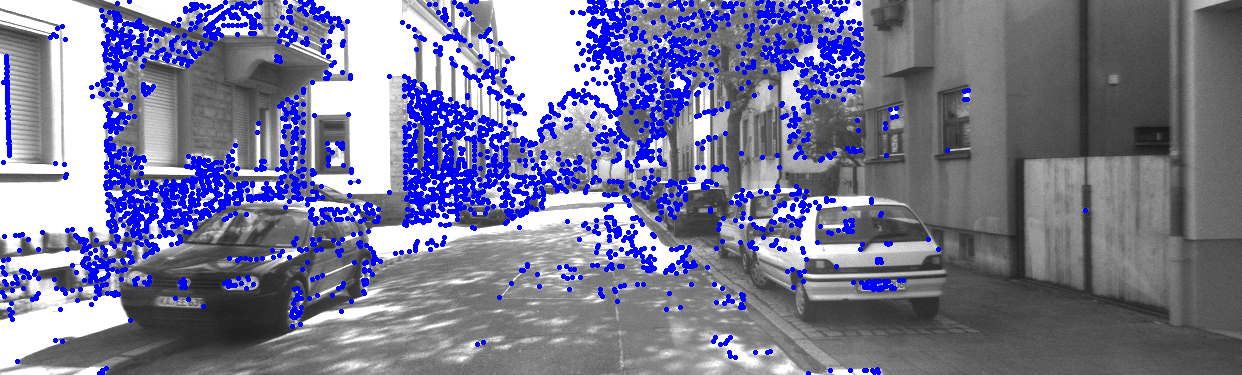
\includegraphics[width=0.75\columnwidth]{./img//harris}\\
(a)\\
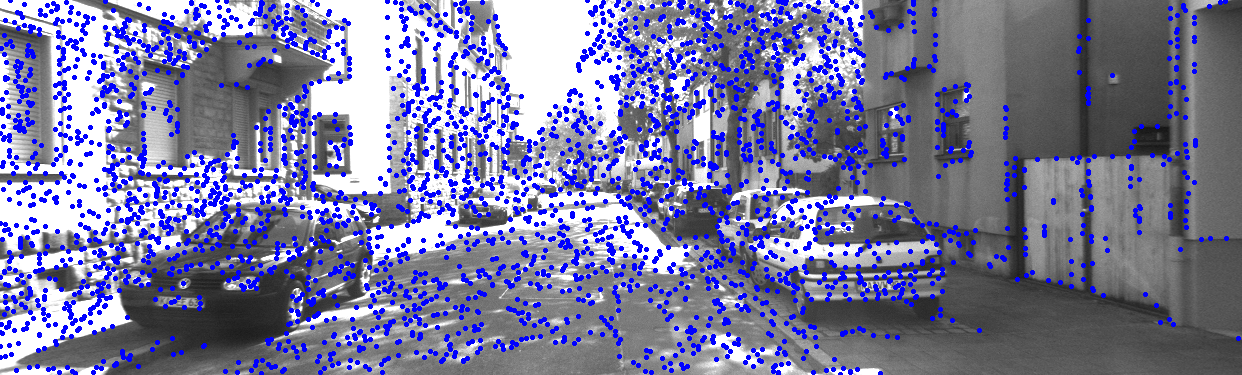
\includegraphics[width=0.75\columnwidth]{./img//edgepoints}\\
(b)\\
\end{tabular}
\caption{Different features extracted on the same image: (a) shows 3609 Harris corners, (b) shows 3595 Edge-Points.}
\label{fig:Edge-Points}
\end{figure}


\begin{figure}
\centering
\begin{tabular}{cc}
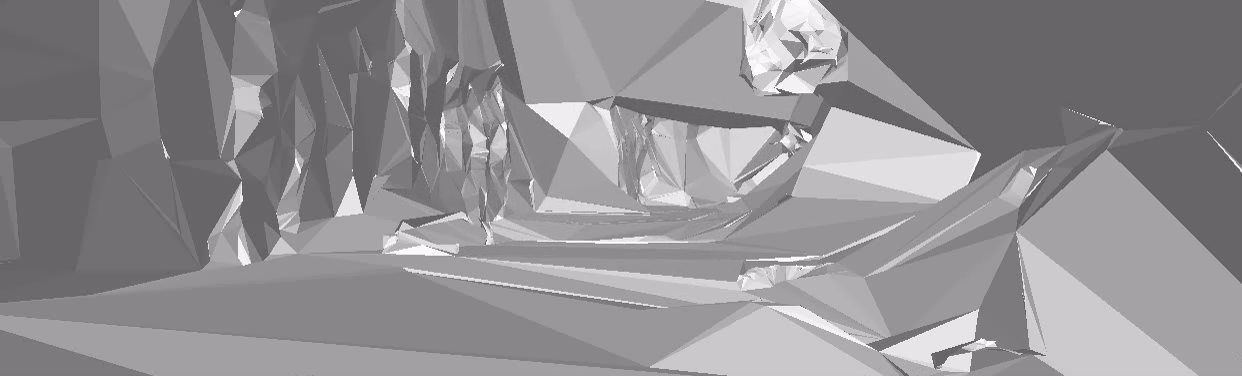
\includegraphics[width=0.75\columnwidth]{./img//reconstrHarris}\\
(a)\\
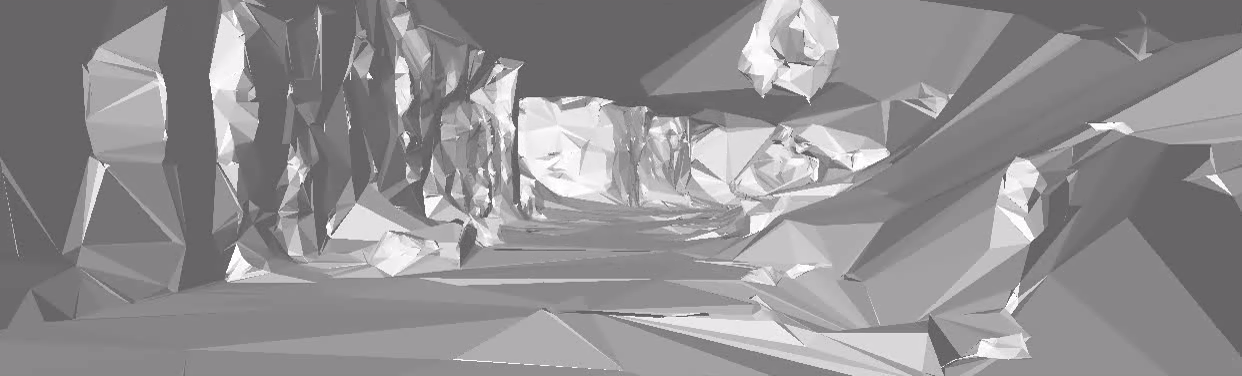
\includegraphics[width=0.75\columnwidth]{./img//reconstr}\\
(b)\\
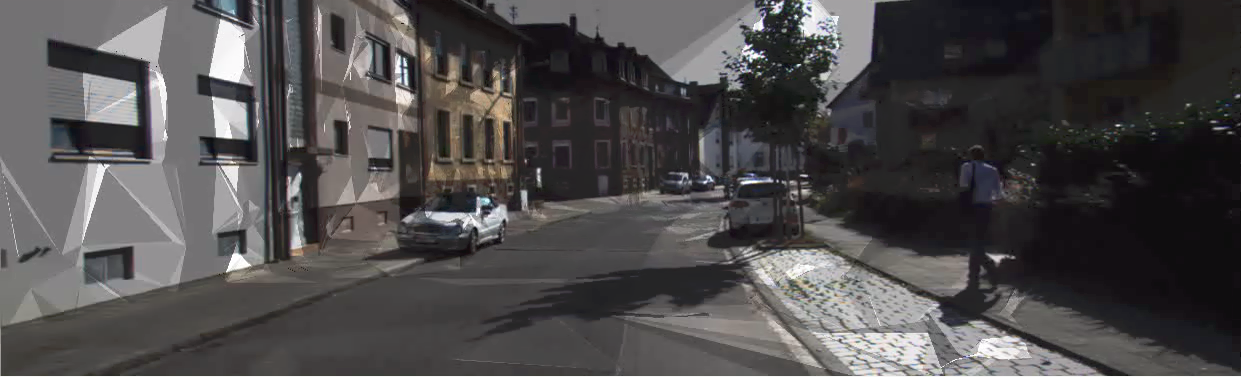
\includegraphics[width=0.75\columnwidth]{./img//reconstrTex}\\
(c)\\
\end{tabular}
\caption{Reconstructions with (a) Harris corners, (b) Edge-Points, and (c) textured reconstruction.}
\label{fig:recons}
\end{figure}

In this paper, we improve on the approach of \cite{litvinov_lhuillier_13} to extract a manifold incrementally. 
Differently from \cite{litvinov_lhuillier_13}, instead of reconstructing 3D points corresponding to Harris features, we propose to build the 3D Delaunay triangulation on the points projecting on the (Canny) edges of the images, named \emph{Edge-Points} (see Fig. \ref{fig:Edge-Points}). 
The existing incremental space carving systems, e.g., \cite{litvinov_Lhiuller14, litvinov_lhuillier_13, Lovi_et_al_11}, rely on sparse point cloud estimated by Structure from Motion, which discards the Edge-Points.

The main drawback of these points is the degree of freedom along the edge itself that usually causes instability in estimation and matching.
Nevertheless, several reasons supports the usage of Edge-Points.
First, urban scenarios show lot of sharp edges, therefore Edge-Points represent suitable vertexes to constrain the edges of the 3D Delaunay triangulation to real-world edges (see Fig. \ref{fig:recons}). 
Then, as Fig. \ref{fig:Edge-Points} shows, Edge-Points provide a better coverage of the image.
Finally, the number of Edge-Points is easier to tune with respect to the classical feature detector: by changing the downsampling rate we change proportionally the number of Edge-Points.

Other authors \cite{Rhein_et_al13, Tomono09} already took advantage of Edge-Points in their systems. Rhein et al. in \cite{Rhein_et_al13} propose a heterogeneous (corner features and Edge-Points) tracker that exploits the epipolar constraint, but, differently from us, their work is focused on the tracking stage and it aims at a sparse point cloud reconstruction.
Tomono \cite{Tomono09}  uses Edge-Points to make  the Simultaneous Localization And Mapping (SLAM) process robust in an indoor scenario that exhibits a lack of texture, but he does not reconstruct the 3D surface of the scene, moreover it uses a stereo rig that makes the estimation of the 3D point positions easier with respect to the monocular case addressed in this paper.

The use of a monocular camera looking forward induces low parallax which makes  the estimation of the 3D point positions not a trivial task. This issue adds to the previously mentioned Edge-Points instability. 
In this paper we show that the combination of the  Kanade-Lucas-Tomasi (KLT) tracker \cite{Lucas_Kanade81}, a convenient filtering of the matches, and Gaussian-Newton optimization successfully handle Edge-Points estimation even in this complex scenario. 

Our system bootstraps from a good estimate of the camera poses, as in many urban 3D reconstruction systems \cite{ Pollefeys_et_al_08, Cornelis_et_al08}. 
We assume the camera pose estimation could be obtained with a Structure from Motion or SLAM technique, e.g., \cite{Snavely_et_al06},  or with an estimate obtained by fusing GPS, inertial sensors and visual odometry such as in \cite{Cucci_Matteucci14}.
This assumption enables us to estimate independently, and very efficiently, the 3D Edge-Point positions.

Besides the use of Edge-Points, a second contribution in this paper addresses the visual artifacts issue that sometimes affects the estimated surface.
This issue was deeply studied in \cite{litvinov_Lhiuller14}, where the authors propose an ad hoc post-processing procedure that attempts to detect and remove the artifacts by preserving the manifold property; it runs quite fast, but its computational complexity is not negligible ($0.43$s per-frame).  
In this paper we propose a very efficient heuristic to preemptively avoid visual artifacts, which runs significantly faster than the previously mentioned procedure (around $0.001$-$0.010$s per-frame). We named this heuristic Inverse Cone Heuristic since the space affected by the heuristic has the shape of a cone directed inversely with respect to camera-to-point viewing ray.

In Section \ref{sec:manifold} we summarize the approach of \cite{litvinov_lhuillier_13} to reconstruct a manifold surface.
In Section \ref{sec:3D-Reconstruction} we describe our incremental reconstruction system, focusing on the 3D Edge-Point cloud estimation and the preemptive approach to remove the visual artifacts. 
In Section \ref{sec:experimental-results} we show the experimental results on the public available dataset KITTI \cite{Geiger_et_al12}, while in Section \ref{sec:conclusion} we conclude the paper.

%----------------------------------------------------------------------------------------------------------------------------
\section{Manifold Reconstruction}%----------------------------------------------------------------------------------
%\subsection{The manifold property}
\label{sec:manifold}
We are interested in reconstructing a manifold surface in the 3D space which represents the observed scene.
A surface is manifold if and only if the surface neighborhood of each point is homeomorphic to a disk.
In the discrete case, the points are the vertexes of the mesh, while the incident triangles (or polygons) form the neighborhood. 
So, a discrete surface is manifold if each vertex $v$ is \emph{regular}, i.e., if and only if the edges opposite to $v$ form a closed path without loops \cite{lhuillier_Yu2013}. 

\subsection{Incremental manifold extraction}
\label{subsec:incrementalManifold_2}
In this section we briefly summarize the method introduced in \cite{litvinov_lhuillier_13} and \cite{litvinov_Lhiuller14}, which, in this paper, we enhance significantly by choosing a proper point cloud to build the Delaunay triangulation and by avoiding most  of the artifacts in the estimated surface with the Inverse Cone Heuristic.

In \cite{litvinov_lhuillier_13}, the authors bootstrap the surface reconstruction from a manifold by partitioning the 3D triangulation of the space between the set $O$ of \emph{outside} tetrahedra, i.e., the manifold subset of the free space (not all free space tetrahedra would be included in this set), and the complementary set $I$ of \emph{inside} tetrahedra, i.e., the remaining tetrahedra that roughly represent the matter.


Let  $\delta( O_{t_{\text{init}}})$ be the initial manifold, i.e., the boundary between $O$ and $I$, estimated as it follows:
\begin{itemize}
  \item \emph{Point Insertion}: add all the 3D points estimated up to time $t_{\text{init}}$ and construct their 3D Delaunay triangulation;
  \item \emph{Ray Tracing}: mark the tetrahedra as free space according to the viewing rays: the list of these tetrahedra is named $F_{t_{\text{init}}}$;
  \item \emph{Growing}: initialize a queue $Q$ with the tetrahedron $\Delta_1 \in F_{t_{\text{init}}}$ that gets the highest number of viewing ray intersections; then iterate the following procedure until $Q$ is empty: (a) remove the tetrahedron $\Delta_{\text{curr}}$ with the highest number of viewing ray intersections from $Q$; (b) add it to $O_{t_{\text{init}}}$ only if the resulting $\delta (O_{t_{\text{init}}} \cap \Delta_{\text{curr}})$  is manifold; (c) add to the queue $Q$ its neighboring tetrahedra that are not already inside the $O_{t_{\text{init}}}$ set. 
\end{itemize}

Once the system is initialized, a new set of points $P_{t_k}$ is generated at $t_k= t_{\text{init}} + k*T_k$, where $k \in \mathbb{N^+}$ is the keyframe index and $T_k$ is the period. 
The insertion of each point $p\in P_{t_k}$ would cause the removal of a set $D_{t_k}$ of the tetrahedra that invalidates the Delaunay property; the surface $\delta (O_{t_k}) = \delta (O_{t_{k-1}} \setminus D_{t_k})$ is not guaranteed to be manifold anymore. 
To avoid this, the authors in \cite{litvinov_lhuillier_13} define a new list of tetrahedra $E_{t_k} \supset D_{t_k}$ and apply the so called \emph{Shrinking} procedure, i.e., the inverse of Growing: they subtract iteratively form $O_{t_{k-1}}$ the tetrahedra  $\Delta \in E_{t_k}$ keeping the manifoldness valid.
After this process, it is likely that $D_{t_k} \cap O_{t_k} = \emptyset$; however, in the case of $D_{t_k} \cap O_{t_k} \neq \emptyset$ the point $p$ is not added to the triangulation.
Once all points in $P_{t_k}$ have been added (or dropped), the \emph{growing} process runs similarly to the initialization procedure, but the queue $Q$ is initialized with the tetrahedra $\Delta \in T \setminus O$ such that  $\Delta \cap \delta O \neq \emptyset$.



%----------------------------------------------------------------------------------------------------------------------------

\section{3D Reconstruction with Edge-Point and Inverse Cone Heuristic}
\label{sec:3D-Reconstruction}
3D reconstruction with space carving entails space discretization.
We choose the 3D Delaunay triangulation to partition the space into tetrahedra since it has been recognized in the literature to be a convenient representation for scene reconstruction \cite{litvinov_lhuillier_13, Pan_et_al09, labatut2007efficient, Lovi_et_al_11}.
In the following we show how we choose and we estimate the sparse point cloud upon which the triangulation is created and how we conveniently carve the space to preemptively avoid artifacts in a novel way that deeply differs from the approach of \cite{litvinov_Lhiuller14}.

%----------------------------------------------------------------------------------------------------------------------------
\subsection{Edge-Points for 3D Delaunay triangulation}
\label{subsec:pcl_estimation}
A key aspect for a 3D reconstruction pipeline, not stressed enough in the literature, is the choice of the points on which the Delaunay triangulation is built, i.e., what kind of points made up the sparse point cloud.

As most of man-made environments, urban scenarios show a lot of sharp edges, e.g., the corners of building fa\c{c}ades, the borders of windows, or the silhouettes of parked cars. Existing 3D space carving systems do not leverage on this information, but they rely only on maximally stable points.
Stable points are suitable features to track, however, a reconstruction relying on them over-simplifies the reconstructed world: it mostly fails to capture the sharp edges which do not show sharp corners too.

We propose to overcome this limitation by estimating the 3D position of Edge-Points, so to constrain the edges of the 3D triangulation to lay close to \emph{real-world} 3D edges. 
This novel triangulation generates a carved space more faithful to the real-world scene, see for instance the difference of the truck of Fig. \ref{fig:reconstrEx}(a) reconstructed with the use of Harris corners in Fig. \ref{fig:reconstrEx}(b), and with the Edge-Points at a low ($\frac{1}{40}$) and high ($\frac{1}{10}$) downsampling rate  in Fig. \ref{fig:reconstrEx}(c) and \ref{fig:reconstrEx}(d) respectively. 

Fig. \ref{fig:Edge-Points} shows that some Edge-Points have been induced by grass and shadows on the road plane. Even if this subset of features will not lay on real-world edges, their presence does not affect the quality of the reconstruction, since they lay, or are close, to the actual \emph{matter}.
Nevertheless most of these points, especially those induced by the grass, get extracted also by the Harris corner detector. 
Let stress one more time here that most of the Edge-Points lay on the real-world edges, while the Harris corners do not locate them very well.
Another important point is that is easy to increment the number of Edge-Points used to reconstruct the environment by keeping the feature quality unchanged, while the corner-like features quality usually degrades as soon as other features are required. 
To verify this, in the experimental section we tested our algorithm with two different downsampling rates showing that the quality of the reconstruction significantly improves as the sampling rate increases. 


\begin{figure}
\begin{center}
\begin{tabular}{cc}
\centering
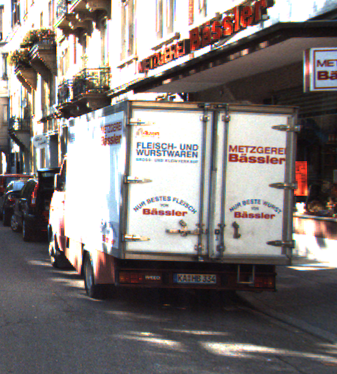
\includegraphics[width=0.3\columnwidth]{./img//imageOrig}&
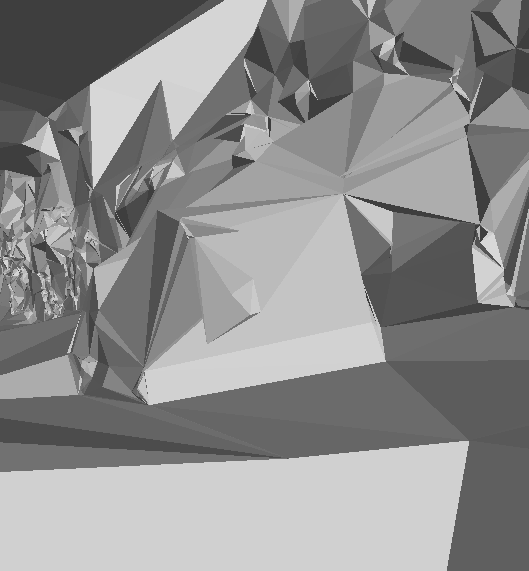
\includegraphics[width=0.3\columnwidth]{./img//notedge}\\
(a) & (b)\\
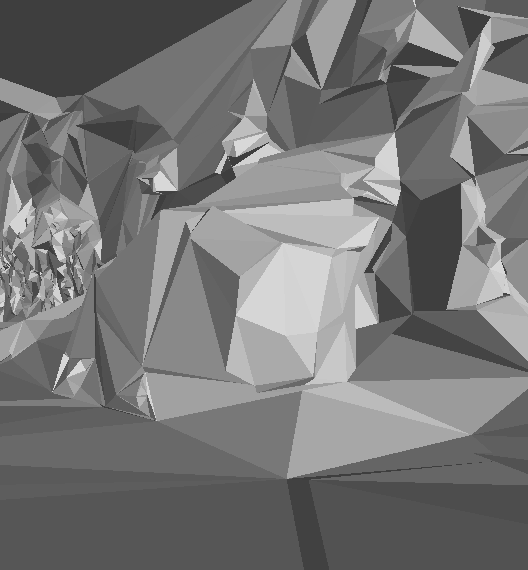
\includegraphics[width=0.3\columnwidth]{./img//edge40}&
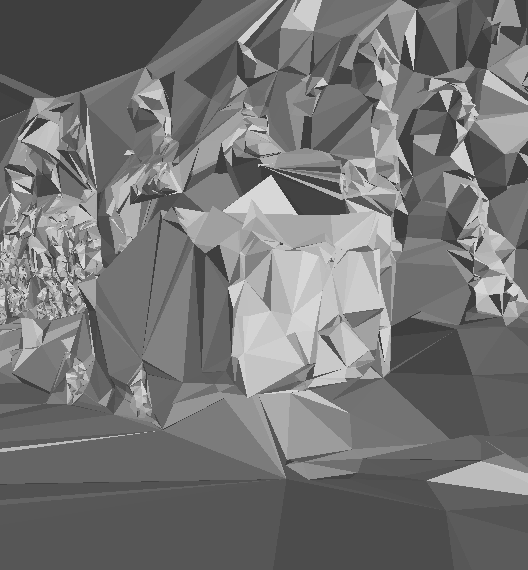
\includegraphics[width=0.3\columnwidth]{./img//edge10}\\
(c) & (d)\\
\end{tabular}
\end{center}
\caption{Three examples of reconstruction from sparse data of the light truck in (a): with Harris corners in (b), with Edge-Points with downsample rate  $\frac{1}{40}$  in (c)  and Edge-Points with  downsample rate  $\frac{1}{10}$ in (d).}
\label{fig:reconstrEx}
\end{figure}


%----------------------------------------------------------------------------------------------------------------------------


\subsection{Edge-Points tracking and reconstruction}
\label{subsubsec:Edge-Point-tracking}
In Fig. \ref{fig:algorithm} we depict the tracking and estimation process.
For each \emph{keyframe}, i.e., one frame every $T_k$, we extract the 2D Edge-Points by (a) estimating the image edges with the Canny algorithm, and (b) downsampling those edges with step $T_{edges}$, i.e., we downsample the chains of pixels that made up the edges. 
Then we track these points in consecutive frames (both in keyframes and non-keyframes). Each \emph{track}, i.e., the sequence of point 2D positions in subsequent images, contains the \emph{measurements} of a 3D point. The value of $T_k$ depends on the camera speed; in our case of surveying vehicle, is fixed such that we have two keyframe per-second. 


We track the 2D Edge-Points with the KLT tracker \cite{Lucas_Kanade81} as suggested by Rhein et al. \cite{Rhein_et_al13} because it enables faster reconstruction with respect to more complex trackers which, for instance, relies on SIFT descriptor computation.
KLT tracks successfully most of the 2D Edge-Points between two consecutive frames; however, to reach good 3D point position estimates, we need to take into account errors due to the low parallax induced by the forward motion of the monocular camera and we need to filter out wrong correspondences produced by the mentioned edge instability. 


The low parallax issue affects the estimation process when the camera looks towards the moving direction. The uncertainty of the 2D point measurement on the image plane is usually assumed to be Gaussian, so the measurement uncertainty spreads in the 3D space, through the uncertainty ellipse on the image plane, as a cone whose vertex is in the camera center. 
When the parallax is low, the uncertainty cones of consecutive measurements of a 3D point are almost overlapped \cite{HaZi04}. As the intersection of these uncertainty cone becomes relevant, the 3D point position estimation is no more reliable.

To ensure  an overall significant parallax and to successfully estimate the 3D points position, we filter the tracks  both at a local and at a global level.
At a local level we filter out an Edge-Point when the displacement of its two consecutive measurements is too small, i.e., when the parallax is almost null and the uncertainty of its estimate tends to infinite. 
We experimentally set this minimum displacement to $d_{meas}^{min} = 5 \text{pixels}$ on our videos, but this parameter is related to the video frame rate and the camera focal length so it should be adapted according to the specific setup. 
Usually, as expected from the forward motion, the points filtered out lay around the center of the image, where the parallax is lower.

At a global level we discard also short tracks, i.e., those tracks containing less then $l_{track}^{min}$ measurements (we recall here that a track is the sequence of measurements of a 3D Edge-Point in subsequent images), where in our setup $l_{track}^{min} = T_K$ (recall that $T_K$ is the keyframe period). 


\begin{figure}[t]
\centering
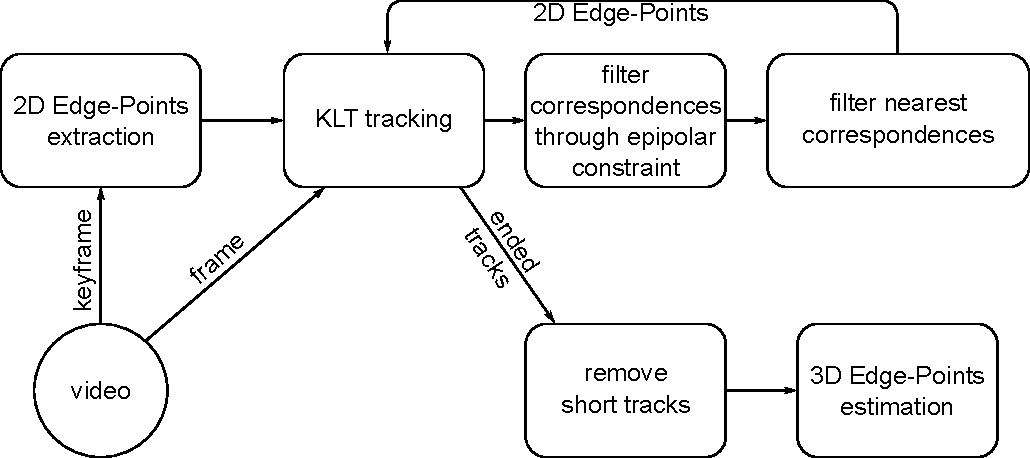
\includegraphics[width=0.8\columnwidth]{./img//EdgePoint}
\caption{Edge-Point tracking and estimation process.}
\label{fig:algorithm}
\end{figure}

To add robustness to the tracking step and manage the well-known instability  of Edge-Points  we drop the correspondences that do not satisfy the epipolar constraint. 
Let $x_{t-1}$ and $x_t$ be two corresponding points in frame $t-1$ and $t$, and $F$ the fundamental matrix between the camera at time $t-1$ and $t$, the following equation holds:
\[
 x_{t-1}^{T}Fx_t = 0 .
\]

Given $K_{t-1}$ and $K_t$ the intrinsic parameters of the two cameras, which are the same in the monocular case, and assuming the world reference frame fixed in camera $t-1$ and $P = [R_t,t_t]$ to be the pose of camera $t$, the fundamental matrix can be computed as:
\[
F = K_t^{-T}R_tK_{t-1}^T [K_{t-1}R_{t}t_t]_x
\]
where $[.]_x$ is the skew-symmetric operator \cite{HaZi04}.
Given a point $x_{t-1}$ and the matrix $F$, the vector $l_{t} = Fx_{t-1}$ is the epipolar line, i.e., the locus of the points corresponding to $x_{t-1}$ in the image plane of camera $t$. 

The epipolar constraint states that, given a point $x_{t-1}$, the corresponding point $x_{t}$ lies on the epipolar line. So, given the KLT correspondence $x_{t-1}$-${x}_{t}$, we drop it if $\text{dist}_{L_2}\{Fx_{t-1}, {x}_{t}\} <\epsilon_e$, where $\epsilon_e$ is fixed to a tolerant value of $\epsilon_e = 20px$ due to the noise of the epipolar contraint estimation induced by the forward motion.
The epipolar constraint represents a necessary, but not sufficient condition. The remaining wrong correspondences will be filtered during the 3D point estimation step.

The previous filtering approach is intended to deal with almost-static scene so it filters out most of  the dynamic objects. This behavior is especially suitable for mapping purposes: in this case the map usually has not to include dynamic object such as moving cars or pedestrians. 

%----------------------------------------------------------------------------------------------------------------------------
\subsubsection*{Parallel 3D Point Positions Estimation}
\label{subsubsec:3D-point-estimation}
Several space carving reconstruction algorithms adopt a Structure from Motion technique to estimate both  the camera pose and the 3D points position at the same time, see for instance \cite{Yu_Lhuillier12, litvinov_lhuillier_13} and \cite{Lovi_et_al_11}. 
On the other hand, in urban applications, especially those involving autonomous vehicles, a very good estimate of the camera pose can be derived from sensors that are different from the camera itself (for instance with the sensor fusion technique in \cite{Cucci_Matteucci14}). 
Therefore, as in  many urban reconstruction systems (\cite{ Pollefeys_et_al_08, Cornelis_et_al08})  we assume the camera pose to be known, while triangulating the 3D edge-points. This assumption allows to estimate the 3D position of each 3D Edge-Point independently, i.e., in parallel.

After the tracking process, for each Edge-Point we first estimate a rough 3D position by triangulating the first and last measurements with the classic algorithm proposed by Hartley and Sturm \cite{Hartley_Sturm97}. 
We then optimize this 3D position estimate with a Gauss-Newton algorithm by minimizing the 3D reprojection error over the whole track (we fixed a number of $N_{GN} = 50$ iterations):
\begin{equation}
 e(X_{3D})^i = P^i \cdot X_{3D} - x_{meas}^i, \forall i \in \text{track}
\end{equation}
where $P^i$ is the $i$-th camera matrix, $X_{3D}$ is the 3D position of the point to be estimated, and $x_{meas}^i$ is the  measurement in the $i$-th image.
Since some wrong correspondence could exist, we drop the Edge-Points for which the mean reprojection error is higher then $\epsilon_{GN} = 2\text{px}$ at the end of optimization.



% 
% \begin{figure}
% \centering
% \begin{tabular}{cc}
% 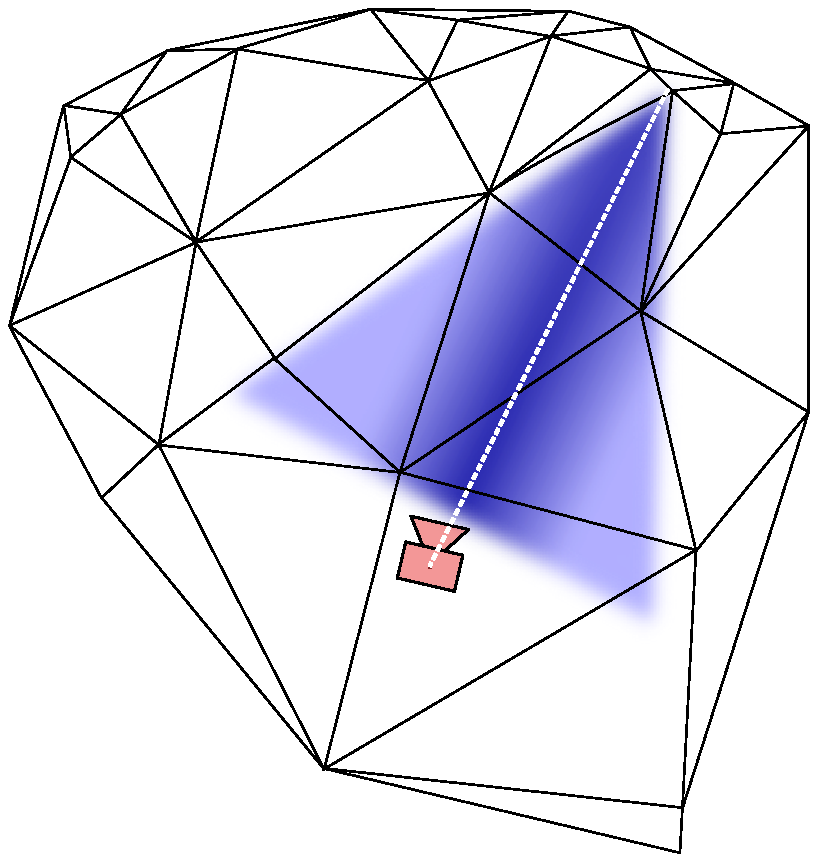
\includegraphics[width=0.45\columnwidth]{./img//conicCarvingContinue}&
% 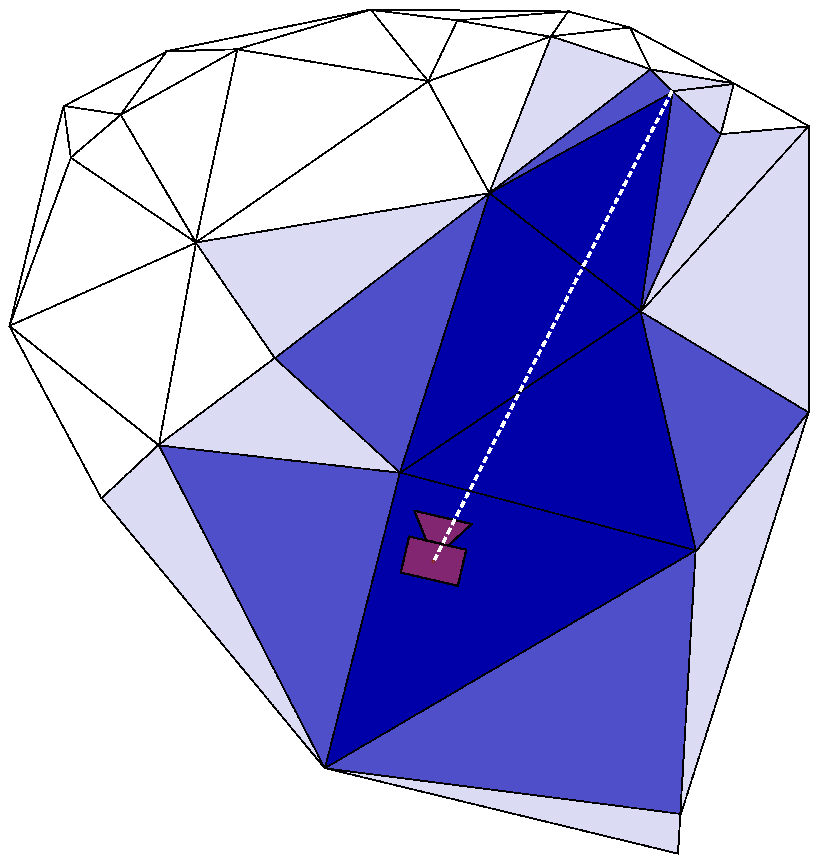
\includegraphics[width=0.45\columnwidth]{./img//conicCarvingImplemented}\\
% (a) & (b)
% \end{tabular}
% \caption{The inverse cone heuristic applied to the ray tracing step. On the left the inverse cone, and on the right our implementation in the Delaunay triangulation domain. Darker blue corresponds to higher weights.}
% \label{fig:ConicCarving}
% \end{figure}

\subsection{Inverse Cone Heuristic for preemptive visual artifacts removal.}
\label{sec:visualartifacts}
%----------------------------------------------------------------------------------------------------------------------------
Once the 3D Edge-Points have been estimated, we propose an enhanced version of the algorithm in \cite{litvinov_lhuillier_13} to reconstruct a manifold surface.
The surface extracted with the algorithm described in Section \ref{sec:manifold} is affected by visual artifacts.
Fig. \ref{fig:artifact} shows a simple scenario where a visual artifacts is generated due to the order of tetrahedra addition to the manifold.
The algorithm bootstraps from the manifold in Fig. \ref{fig:artifact}(a); then it grows the manifold by we add the triangle A (Fig. \ref{fig:artifact}(b)). Afterward, C and D are free space but they are kept in the inside set, otherwise they invalidate the manifold property; this two triangles make up a visual artifact.

In our case the visual edges which are critical for the reconstruction quality are those containing at least one edge long enough to be considered unrealistic. 
More formally, Litvinov and Lhuiller, in \cite{litvinov_Lhiuller14}, define a \emph{critical visual artifact} as a set of tetrahedra belonging to the free space, but not included in the outside set and which contains at least one \emph{visually critical edge}, i.e., an edge $ab$ such that exists a camera center $c$ such as $\widehat{acb}>\alpha$, where $\alpha$ is a user defined parameter (in our algorithm we do not need to define this parameter).
\begin{figure}
\centering
\begin{tabular}{cc}
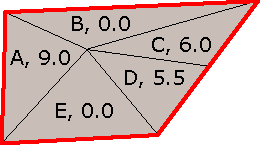
\includegraphics[width=0.35\columnwidth]{./img//artifacts01}&
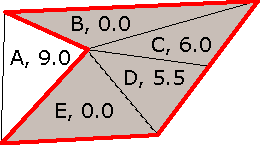
\includegraphics[width=0.35\columnwidth]{./img//artifacts02}\\
(a) & (b)
\end{tabular}
\caption{Simple scenario where a visual artifact is generated. Each triangle is labelled as ``name, weight''. The bold red line is the boundary between inside (dark triangles) and outside (white triangles) sets. Bootstrapping from (a), the triangle A is added to the manifold in (b), then neither C or D can be added anymore without invalidating the manifold property.}
\label{fig:artifact}
\end{figure}


\begin{figure}
\centering
\begin{tabular}{cc}
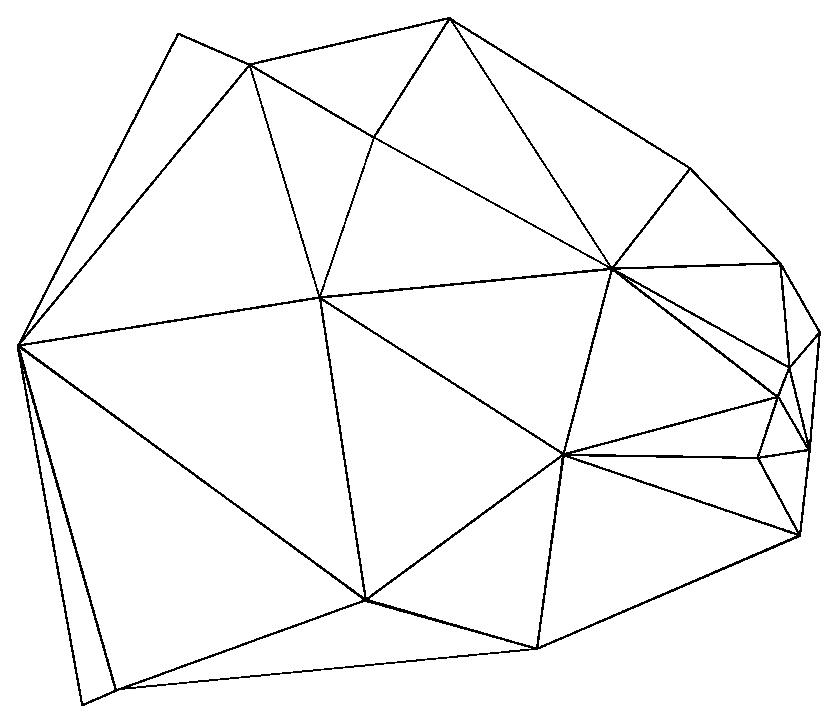
\includegraphics[width=0.35\columnwidth]{./img//conicCarvingContinueOK}&
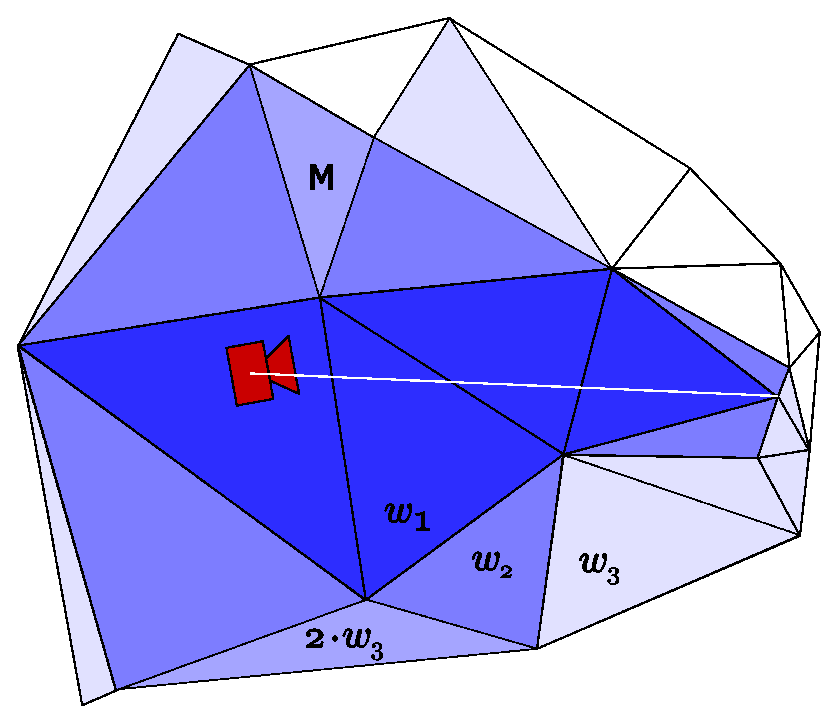
\includegraphics[width=0.35\columnwidth]{./img//conicCarvingOK}\\
(a) & (b)
\end{tabular}
\caption{The inverse cone heuristic applied to the ray tracing step. On the left the inverse cone, and on the right our implementation in the Delaunay triangulation domain. Darker blue corresponds to higher weights.}
\label{fig:ConicCarving}
\end{figure}


Litvinov and Lhuiller in \cite{litvinov_Lhiuller14}, propose a post-processing method to detect and remove critical artifacts keeping the manifold property valid.
In this paper, we propose a preemptive approach significantly different, and complementary, with respect to \cite{litvinov_Lhiuller14}. 
Our idea relies on two observations: the tetrahedra that likely turn into visually critical edges are big tetrahedra since they contains long edges, and big tetrahedra are mostly close to the camera path.

As the example of Fig. \ref{fig:artifact} shows, the order of growing is a key point to avoid the creation of visual artifacts; thus,
 by modifying the ray tracing step, we aim preemptively enforce a carving order such that big tetrahedra near to the camera become the first to be added to the reconstructed manifold.
We replace the intersection count associated to each tetrahedron with a weight. Ideally in the continuous space, we would apply  a cone-shaped weighting heuristic, we named Inverse Cone Heuristic, which opens inversely with respect to the ray sense (see Fig. \ref{fig:ConicCarving}(a)),  such that the region receiving weights increments gets smaller and smaller as the ray approach the viewed point.
In the real discrete implementation, for each ray from the camera to the 3D point, we increment by $w_1$ the weights of the traversed tetrahedra, by $w_2$ the weights of their neighbors and by $w_3$ the weights of the neighbors of the latter tetrahedra.
Since big tetrahedra are near to the camera, this induces the cone-shaped weighting scheme as in Fig. \ref{fig:ConicCarving}(b).

As Fig. \ref{fig:ConicCarving}(b) shows, some ``neighbors of neighbor'' tetrahedra receive more than one increment, in particular they receive up to 4 multiple increments (one for each neighbor), but in practical cases they are usually 2 or 3.
Multiple increments let to spread the weights to tetrahedra close to the ray, without any  neighboring facet to the traversed tetrahedra, e.g.,  triangle M in Fig. \ref{fig:ConicCarving}(b).
To avoid high weights due to multiple increments, we tune the value of $w_3$ such that the maximum increment for neighbors of neighbor is equal to $w_2$.
For all the datasets we fixed $w_1$ to a reference value of $1.0$, then $w_2$ to a close value of $0.8$ and $w_3 = \frac{w_2}{4} = 0.2$, where 4 represents the maximum number of multiple increments received by one tetrahedra for a single ray. 


After the ray tracing step, the region growing and shrinking procedures follows the ordering induced by the computed weights, but, to avoid carving the actual matter, one tetrahedron is added, or subtracted, to the manifold only if is traversed by at least one camera-to-point ray.










\section{Manage the moving points}
\section{Introduction}
\label{sec:intro_ch5b}
Incremental 3D reconstruction from a sparse point cloud is gaining interest in the computer vision community as incremental Structure from Motion algorithms are consolidating  \cite{wu13}. 
This is clearly true for those applications where a rough, but dense, surface represents a sufficient and effective representation of the scene, e.g, for traversability analysis in unmanned vehicle navigation. 
Furthermore, in real-time applications, the map of the environment needs to be updated online, and the surface has to be estimated incrementally. 

Most of the existing algorithms \cite{Lovi_et_al_11,Pan_et_al09,litvinov_lhuillier_13,litvinov_Lhiuller14} bootstrap the reconstruction of a mesh surface from the 3D Delaunay triangulation of a sparse point cloud. Indeed, the 3D Delaunay triangulation  is very powerful:
the Delaunay property, i.e., no point of the triangulation is inside the sphere circumscribing any tetrahedron, avoids as much as possible the resulting tetrahedra to have a degenerate shape \cite{Maur_02}; it is self-adaptive, i.e., the more the points are dense the more the tetrahedra are small; it is very fast to compute, and to  update against point removal or addition; off-the-shelf libraries, such as CGAL \cite{cgal}, enable a very simple and efficient management of it. 

As soon as a Delaunay triangulation is available, several approaches exist to extract a surface taking into account the visibility of each point. 
The simplest algorithm is the Space Carving \cite{Kutulakos_Seitz05}: it initializes all the tetrahedra as \emph{matter}, then it marks as \emph{free space} the tetrahedra intersected by the camera-to-point \emph{viewing rays}, i.e., the lines from the camera center to the observed 3D points in the triangulation. 
The boundary between free space and matter represents the final surface of the scene.
Pan et al. \cite{Pan_et_al09} improve upon this simple procedure by proposing an online probabilistic Space Carving, but this is not an incremental approach: they start from scratch every time new points are added.
Lovi et al. \cite{Lovi_et_al_11} present the first incremental Space Carving algorithm which runs real-time, but, as for the previous methods, the estimated surface is not guaranteed to be manifold 

Several reasons lead to enforce the manifold property as explained in \cite{lhuillier20152}. 
Most Computer Graphics algorithms need the manifold property, for instance smoothing with Laplace-Beltrami operator \cite{Meyer03}, or the linear mesh parametrization \cite{saboret00}.
Moreover the manifold property enables surface evolution in mesh-based Multi-View Stereo, as in \cite{vu_et_al_2012,delaunoy_et_al_08}.the manifold property enables a photometric refinement by surface evolution such as with the high accurate Multi-View Stereo mesh-based algorithm as in \cite{vu_et_al_2012,delaunoy_et_al_08}.
With these approaches is hard to estimate the surface evolving flow in the presence of non manifold vertices: indeed they compute for each vertex the gradient minimizing the reprojection error, by summing-up the contribution of the incident facets; if the vertex is not manifold, this gradient does not converge. As a further proof of this, \cite{vu_et_al_2012} needs to manually fix the surface estimated via s-t cut.
As in \cite{vu_et_al_2012}, it is possible to fix the mesh as a post-processing step, but reconstructing directly a manifold as in the proposed paper, enables the design of a fully automatic pipeline which do not need human intervention.

In literature, the only algorithm reconstructing a manifold incrementally was proposed by Litvinov and Lhuiller \cite{litvinov_lhuillier_13,litvinov_Lhiuller14}. 
In their work, the authors  bootstrap from the Space Carving procedure and, by taking into account the number of intersections of each tetrahedron with the viewing rays, they reconstruct a surface keeping the manifold property valid. 
The main limitation is that  Litvinov and Lhuiller insert a point into the Delaunay triangulation only when its position is definitive, then they cannot move the point position anymore even in the case they could refine their estimate. 
The main reason of Litvinov and Lhuiller design choice has to be ascribed to the computational cost of updating the visibility information along the viewing rays incident to each moved point, and the computational cost of updating part of the Delaunay triangulation, which in turn induces a new manifold reconstruction iteration step.

Indeed, the very common approach to deal with a point moving in the triangulation, is to remove it and add it back in the new position \cite{cgal} (Fig. \ref{fig:moving_ch5}). 
When we remove a point (the point A in Fig. \ref{fig:moving_ch5}(a)) and we want to keep the Delaunay property, we have to remove all the tetrahedra incident to that point (light red triangles in Fig. \ref{fig:moving_ch5}(b)); then, we add a new set of tetrahedra to triangulate the resulting hole (dark green triangles in \ref{fig:moving_ch5}(c)).
When we add a new point into the triangulation  (the point B in Fig. \ref{fig:moving_ch5}(d)), a set of tetrahedra would conflict with it, i.e., the Delaunay property is broken (light red triangles in Fig. \ref{fig:moving_ch5}(d)); so, we remove this set of tetrahedra again (red triangles in Fig. \ref{fig:moving_ch5}(e)) and we add a new connected set that re-triangulate the hole (dark green triangles in Fig. \ref{fig:moving_ch5}(f)).
Whenever a set of tetrahedra is replaced, we have to transfer conveniently the information about the visibility (matter or free space) of the removed tetrahedra to the new one. 
In addition to this, we have to update the visibility of the tetrahedra crossed by a visibility ray from one camera to the moved point.
For these reasons the update of the point position is computational demanding.

To complete the overview of the incremental reconstruction methods from sparse data, we mention here another very different approach was proposed by Hoppe et al. \cite{Hoppe13} who label the tetrahedra with a random field, and extract the surface via graph-cuts by minimizing a visibility-consistent energy function. This incremental algorithm is effective and handles the moving points, but the manifold property of the reconstructed surface is not yet guaranteed.

\begin{figure}[t]
\centering
\begin{tabular}{cccccc}
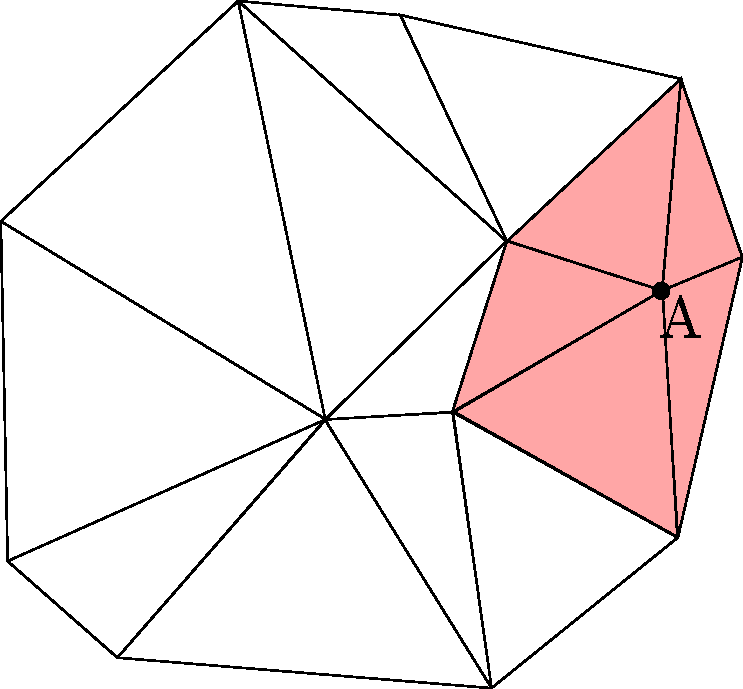
\includegraphics[width=0.13\columnwidth]{./img//delaunayExampleMoving01}&
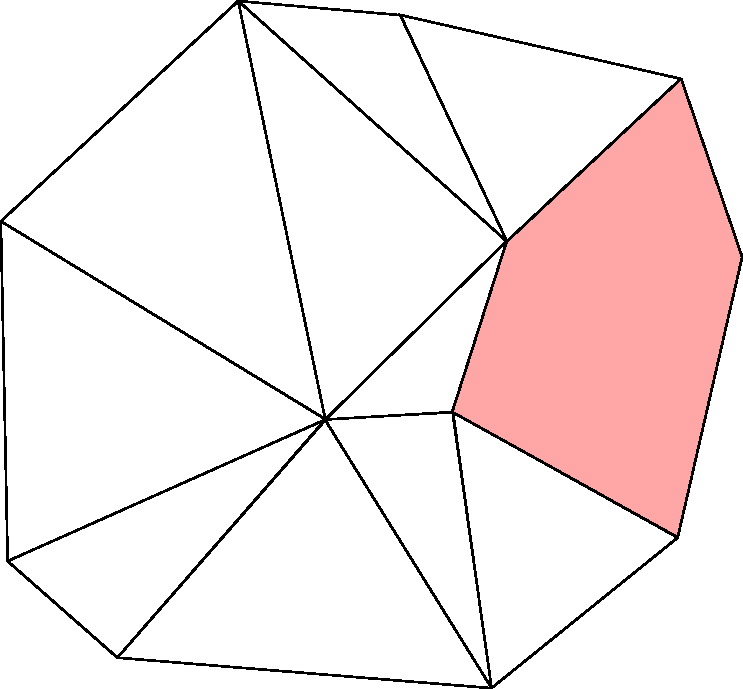
\includegraphics[width=0.13\columnwidth]{./img//delaunayExampleMoving02}&
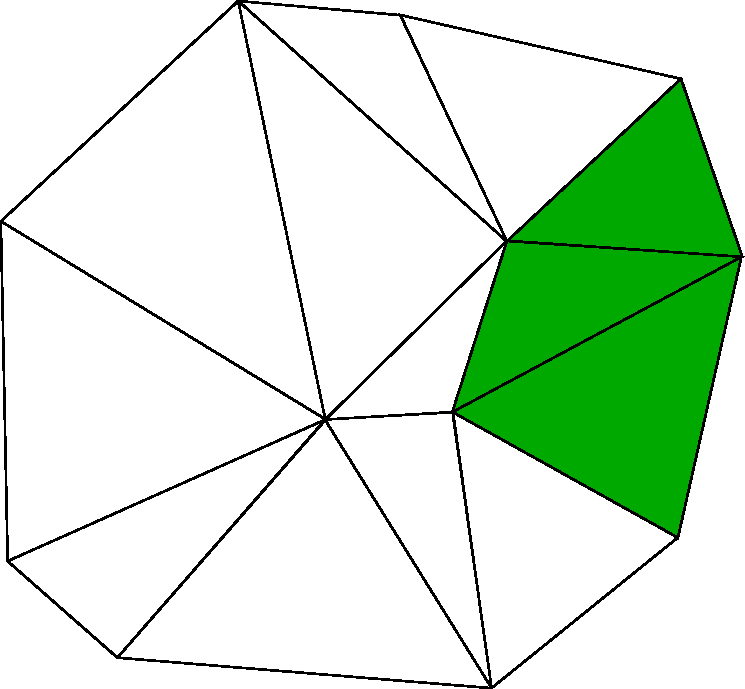
\includegraphics[width=0.13\columnwidth]{./img//delaunayExampleMoving03}&
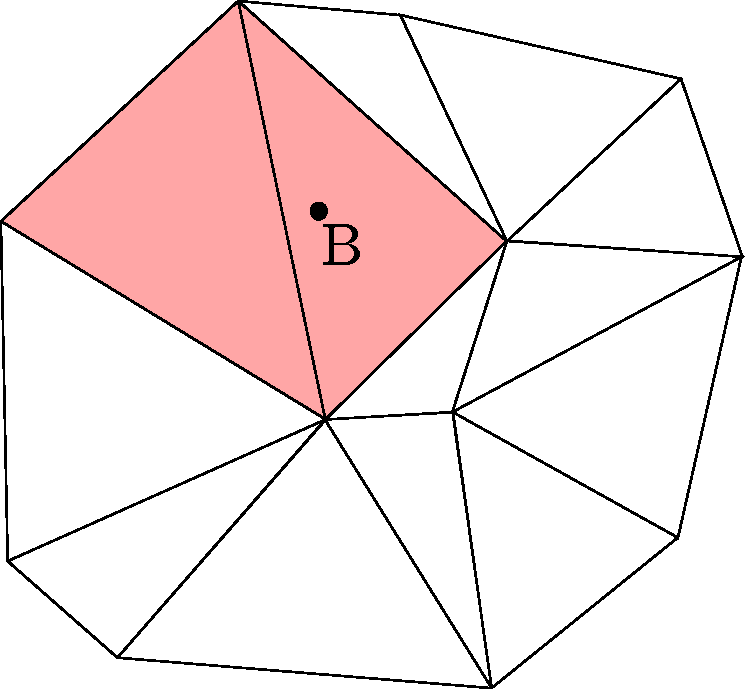
\includegraphics[width=0.13\columnwidth]{./img//delaunayExampleMoving04}&
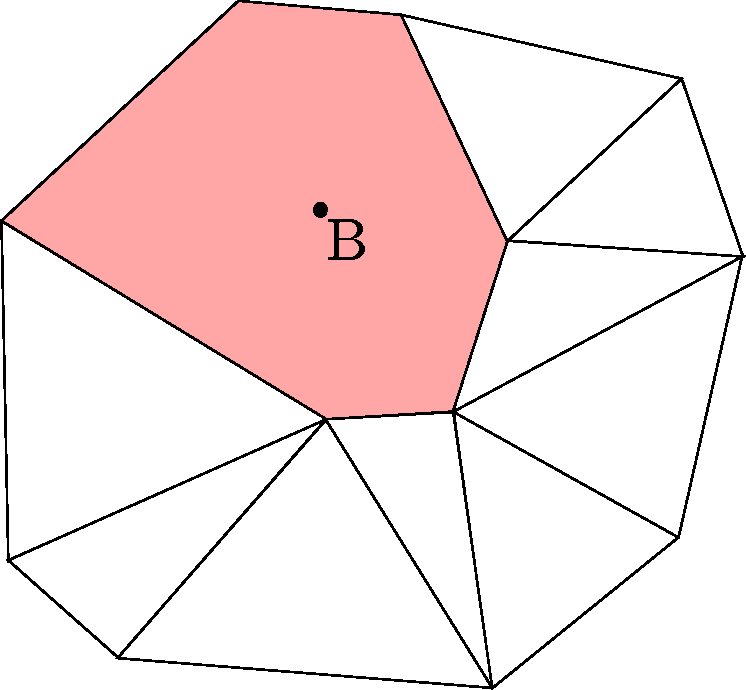
\includegraphics[width=0.13\columnwidth]{./img//delaunayExampleMoving05}&
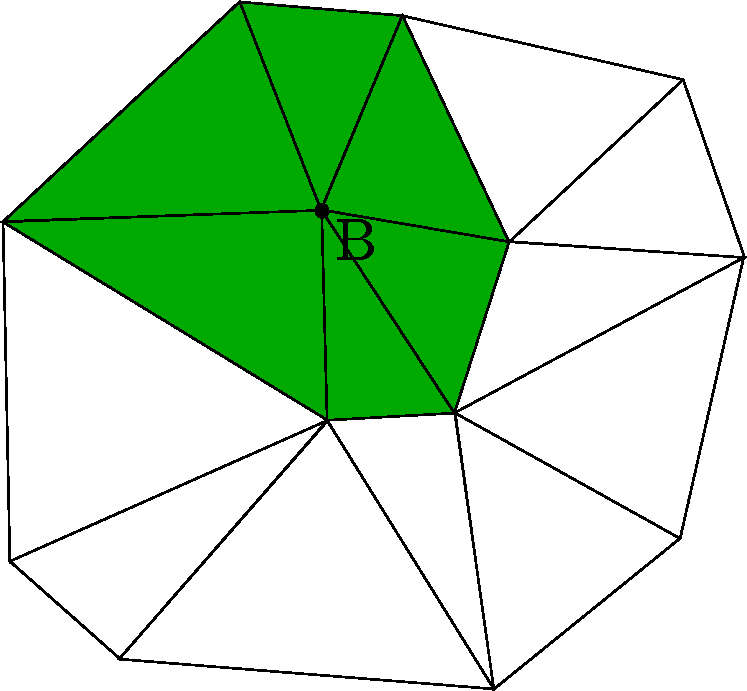
\includegraphics[width=0.13\columnwidth]{./img//delaunayExampleMoving06}\\
(a)&(b)&(c)&(d)&(e)&(f)
\end{tabular}
\caption{Example of point removal in 2D case. Light red triangles depict are removed and replaced with the new dark green ones.}
\label{fig:moving_ch5}
\end{figure}

In this paper we propose, to the best of our knowledge, the first manifold 3D reconstruction algorithm from sparse data which deals with dynamic point changes. In particular, we  show that in this setting the algorithm by Lovi et al. \cite{Lovi_et_al_11} provides a feasible solution, but it is very inefficient and we propose a novel efficient policy to handle the visibility update of Delaunay tetrahedra with moving points. 

In Section \ref{sec:manifold_2} we summarize a slightly modified version of the approach of \cite{litvinov_lhuillier_13} we use to reconstruct a manifold surface.
In Section \ref{sec:3D-Reconstruction_2} we describe Lovi's approach \cite{Lovi_et_al_11} and our proposal to deal with moving points, together with a complexity analysis that explains why our approach is more efficient. 
In Section \ref{sec:experimental-results} we show the experimental results on the publicly available dataset KITTI \cite{Geiger_et_al12}, while, in Section \ref{sec:conclusion} we point out some future works and in  the conclusion of the paper.

%----------------------------------------------------------------------------------------------------------------------------
\section{Manifold Reconstruction} %----------------------------------------------------------------------------------
\label{sec:manifold_2}
In this paper we reconstruct a manifold surface that represents the observed scene. 
A surface is manifold if and only if the neighborhood of each point is homeomorphic to a disk. 
In the discrete case, the points are the vertexes of a mesh, and the neighborhood is represented by the incident triangles (or polygons); a surface is manifold if each vertex $v$ is \emph{regular}, i.e., if and only if the edges opposite to $v$ form a closed path without loops  (see \cite{litvinov_lhuillier_13} for more details). 

% We show in Fig. \ref{fig:vertexManifold} (a) one example of regular vertex and in Fig. \ref{fig:vertexManifold}(b) and \ref{fig:vertexManifold}(c) two cases when the vertex is not regular and thus it breaks the manifold property.
% 
% 
% \begin{figure}[t]
% \centering
% \begin{tabular}{ccc}
% 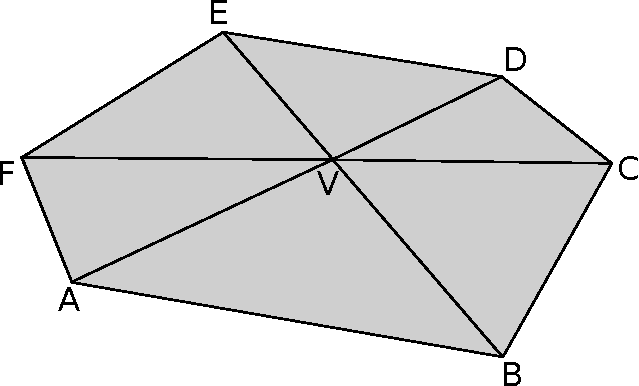
\includegraphics[width=0.25\columnwidth]{./img//manifold}&
% 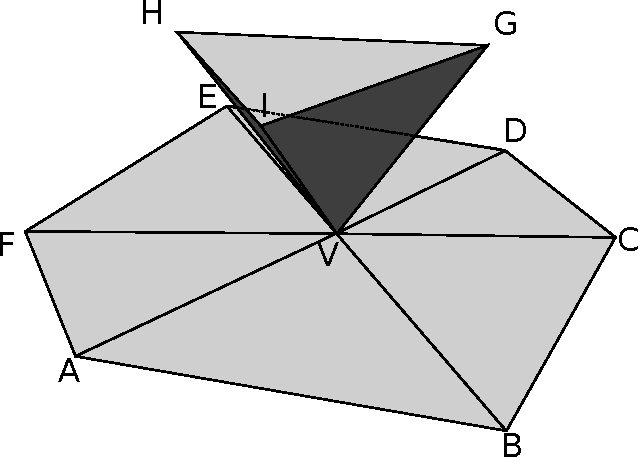
\includegraphics[width=0.25\columnwidth]{./img//notmanifold1}&
% 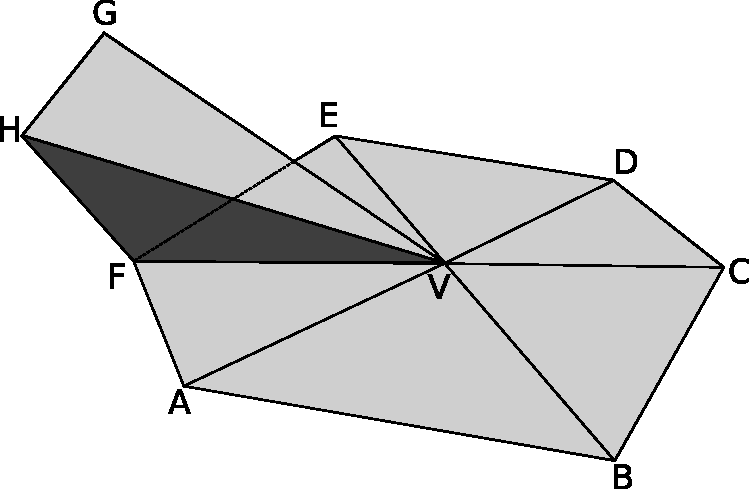
\includegraphics[width=0.25\columnwidth]{./img//notmanifold2}\\
% (a)&(b)&(c)
% \end{tabular}
% \caption{The manifold property: the vertex $V$ in (a) is regular ($ABCDEF$ is a closed path without cycles); the vertex $V$ in (b) and (c) is not regular (in (b) the path $ABCDEFGHI$ is not closed, and in (c) $ABCDEFGHF$ has two cycles).}
% \label{fig:vertexManifold}
% \end{figure}


\subsection{Incremental manifold extraction with tetrahedra weighting}
\label{subsec:incrementalManifold}

In this section we briefly summarize our variation on the method originally proposed in \cite{litvinov_lhuillier_13} enhanced by a weighting scheme that avoids the creation of most visual artifact in the final mesh (more discussion about visual artifacts in \cite{litvinov_Lhiuller14}).  
In our Space Carving algorithm, a weight roughly represents how many rays intersect a tetrahedron, and in the following, a tetrahedron belongs to \emph{free space} if its weight $w$ is higher than a threshold $T_w$ (in our case $T_w = 1.0$).

\subsubsection{Sparse point cloud}
The input of our algorithm is a sparse 3D point cloud, estimated incrementally by assuming the camera poses to be known.
For each keyframe, i.e., every $K=5$ frames, we extract Edge-point features, i.e. 2D points laying on the image edges \cite{Rhein_et_al13}; these points represent measurements of 3D points.
Frame-by-frame we track these features with the Kanade-Lucas-Tomasi tracker, and, at each keyframe, we estimate the new positions of the 3D points with the new  measurements available from the tracking. New estimates are obtained by triangulating the 2D tracked points and by minimizing the reprojection error with a Gauss-Newton algorithm. Once a new estimate of a 3D point is available, we add it to the Delaunay triangulation, i.e., to the reconstruction; then we update its position according to the new measurements: this update induces the motion of the points inside the triangulation.

\subsubsection{3D reconstruction}
The reconstruction of the surface bootstraps from the manifold partitioning the 3D triangulation between the set $O$ of \emph{outside} tetrahedra, i.e., the manifold subset of the free space (not all the free space tetrahedra will be part of the manifold), and the complementary set $I$ of inside tetrahedra, i.e. the remaining tetrahedra that represent the matter together with the free space tetrahedra which would invalidate the manifold property.

Let  $\delta (O_{t_{\text{init}}})$ be the initial manifold. This initial manifold is obtained with the following steps. \emph{Point Insertion}: add all the 3D points estimated up to time $t_{\text{init}}$ and build thir 3D Delaunay triangulation. \emph{Ray tracing and tetrahedra weighting}: for each viewing ray, the algorithm traverses the triangulation and adds a weight $w_1 = 1.0$ to the intersected tetrahedra, a weight $w_2 = 0.8$ to the neighbors and a weight $w_2 = 0.2$ to the neighbors of their neighbors. 
Such weighting scheme acts as a smoother of the visibility and avoids the creation of visual artifacts; it is the main difference between our algorithm and the algorithms proposed in \cite{litvinov_lhuillier_13,litvinov_Lhiuller14}. \emph{Growing}: initialize a queue $Q$ starting from the tetrahedron with the higher weight. Then: (a) pick  the tetrahedron with highest weight from $Q$ and add it to $O_{t_{\text{init}}}$ only if the resulting surface between $O_{t_{\text{init}}}$ and $I_{t_{\text{init}}}$ remains manifold; (b) if inserted  add the neighboring tetrahedra to the queue $Q$, otherwise discard it; continue iteratively until $Q$ is empty.

Once the system is initialized, a new set of points $P_{t_k}$ is estimated at each $t_k= t_{\text{init}} + k*T_k$ frame, named keyframes, where $k \in \mathbb{N^+}$ and $T_k$ is the inverse of the keyframe rate. 
The insertion of a point $p\in P_{t_k}$ causes the removal of the set $D_{t_k}$ of tetrahedra breaking the Delaunay property, and, the surface $\delta (O_{t_k}) = \delta (O_{t_{k-1}} \setminus D_{t_k})$ is not guaranteed to be manifold anymore. 
To avoid this, the authors in \cite{litvinov_lhuillier_13} define a list of tetrahedra $E_{t_k} \supset D_{t_k}$ and apply the \emph{Shrinking} procedure, i.e., the inverse of Growing:  they subtract iteratively from $O_{t_{k-1}}$ the tetrahedra  $\Delta \in E_{t_k}$ keeping the manifoldness valid.
After this process, it is likely that $D_{t_k} \cap O_{t_k} = \emptyset$. Whenever $D_{t_k} \cap O_{t_k} \neq \emptyset$ the point $p$ is not added to the triangulation, i.e., is dropped.
Once all points in $P_{t_k}$ have been added (or dropped), the growing process runs similarly to the initialization procedure, but the queue $Q$ is initialized with the tetrahedra $\Delta \in T \setminus O$ such that  $\Delta \cap \delta O \neq \emptyset$.

%----------------------------------------------------------------------------------------------------------------------------
\section{Reconstructing a manifold with moving points}
\label{sec:3D-Reconstruction_2}
As previously described, Litvinov and Lhuiller \cite{litvinov_lhuillier_13} algorithm adds points to the triangulation only when their 3D position is completely defined; by doing this, there are no changes in the Delaunay triangulation, induced by moving points. This  results in a restriction if we would like to refine the estimation of the position of a point 3D position after its insertion.

Only Lovi et al. \cite{Lovi_et_al_11} presents an incremental Space Carving algorithm which deals with moving points, but their method does not enforce the manifold property.
In this paper we verify the approach of Lovi et al. \cite{Lovi_et_al_11} to be very inefficient for manifold reconstruction, and we present a different approach to deal with moving points that leads to a significant faster computation.


\subsection{The straightforward approach}
\label{subsec:straightforward_way}
The simplest way to deal with moving points while reconstructing a manifold surface, is to apply a straightforward modification to the so called \emph{Refinement Event Handler} by Lovi et al. in \cite{Lovi_et_al_11}.
The Refinement Event Handler algorithm assumes that, for each tetrahedron in the Delaunay triangulation a list of the intersecting viewing rays is stored. In our voting schema an intersecting ray is each ray that increase the weight of the tetrahedron. 

Let $p_{\text{old}}$ be a point that moves to position $p_{\text{new}}$, the algorithm in \cite{Lovi_et_al_11} moves the point by removing point $p_{\text{old}}$ and adding $p_{\text{new}}$ as a new point, according to the classical approach of \cite{Devillers03}, then for each point they apply the following steps. \emph{Rays collection}: collect in a set $U$ all the rays stored into the tetrahedra incident to $p_{\text{old}}$, i.e., those affected by the $p_{\text{old}}$ removal (e.g., the light red triangle in Fig. \ref{fig:moving_ch5}(a)). \emph{Vertex removal}: remove the vertex $p_{\text{old}}$ and its neighboring tetrahedra from the triangulation (Fig. \ref{fig:moving_ch5}(b)); then re-triangulate the hole left by the deleted tetrahedra (Fig. \ref{fig:moving_ch5}(c)). \emph{New point insertion}: insert the new point $p_{\text{new}}$ into the triangulation and add to the set $U$ all the rays stored in the conflicting tetrahedra (Fig. \ref{fig:moving_ch5}(d-f)). \emph{Rays removal}: for each tetrahedron of the entire triangulation remove the rays ending in $p_{\text{old}}$. \emph{Ray casting}: cast one ray for each ray in $U$.

In our case, whenever the 3D estimate of a point moves, we apply the Refinement Event Handler, before point addition and region growing, if and only if the point is inside the shrinked volume $D_{t_k}$ (see Section \ref{sec:manifold}), otherwise we do not move the point (this second case happens very rarely \cite{litvinov_lhuillier_13}).
\subsubsection{Complexity}
The number of rays involved in space carving algorithms is $O(F\cdot N^2)$ where $F$ and $N$ represent respectively the number of frames and the number of points in the triangulation \cite{Lovi_et_al_11}, and the number of tetrahedra in a 3D triangulation grows quadratically with the number of points ($O(N^2)$). 
In Table \ref{tab:ComStraight} we reported the complexities for each of the previous stage; since our implementation exploits the CGAL \cite{cgal} 3D triangulation data structure, the complexity of a single Ray casting, i.e., a cast of a single ray, is $O(N)$ in the general case, but we bound the size of the viewing ray, to avoid to include too far uncertain 3D points estimates, so the final complexity becomes $O(1)$  (see \cite[p.94]{yu2013automatic}).

From the analysis in the table is quite clear that this straightforward solution is not scalable, especially for the dependence between the number of rays and the number of processed frames. 

\begin{table}[t]
\caption{Complexity analysis; \emph{``-''} means not existing step.}
\label{tab:ComStraight}
\scriptsize
\centering
\begin{tabular}{lcccc}
\toprule 
Step                & straightforward     & K  & proposed     & window \\
                    & algorithm & heuristic & algorithm & heuristic \\
\midrule
Rays collection     &  $O(F\cdot N^2)$ & $O(N)$ &-&-\\
Weight collection    &-&- &  $O(N)$ & $O(N)$ \\
Vertex Removal      &  $O(N)$           & $O(N)$ &  $O(N)$           & $O(N)$ \\
New points insertion&  $O(F\cdot N^2 \cdot N)$ & $O(N)$ &  $O(F\cdot N^2 \cdot N)$ & $O(N)$ \\
Rays removal     &  $O(N^2\cdot F\cdot N^2)$ & $O(N^2)$ &-&-\\
Weight Update     &-&-&  $O(N)$ & $O(N)$ \\
Backward ray casting &-&-    &  $O(N^2\cdot F)$ & $O(N)$ \\
Ray casting     &  $O(N^2\cdot F)$ & $O(1)$ &  $O(N^2\cdot F)$ & $O(1)$ \\
\midrule
Overall complexity     &  $O(N^4\cdot F)$ & $O(N^2)$ &  $O(N^3\cdot F)$ & $O(N)$ \\
\end{tabular}
\end{table}

\subsubsection{Forgetting Heuristic}
Lovi et al. \cite{Lovi_et_al_11} proposed a \emph{forgetting} heuristic to limit the number of rays stored in each tetrahedron to a fixed number $K$, thus making the complexity independent from the number of the processed frames. 
However, we show in Section \ref{sec:experimental-results} that, when the points are moving,  the reconstruction is very inefficient even with this heuristic.

\subsection{The efficient approach}
\label{subsec:efficient_way}
%----------------------------------------------------------------------------------------------------------------------------
Our contribution in this paper is an approach to deal with moving points, different from the straightforward variation of \cite{Lovi_et_al_11}. Indeed in our proposal, we avoid storing the list of rays inside each tetrahedron, and we just store the weight associated with it.
This allows the incremental reconstruction algorithm of Section \ref{subsec:incrementalManifold}, and, at the same time, we are able to bound the temporal complexity.

The main difficulty in the proposed approach is updating coherently the weights whenever a point moves, i.e., when the point is removed from the triangulation and added as a new point. As soon as the point is removed from the triangulation, we perform a backward ray casting with negative weights for each viewing camera such that the influence of the point is neglected. Then we remove the point, and we add a new vertex in the new position. Finally, we perform the ray casting from each viewing camera to the new point.

During both point removal and addition, we have to remove a set of connected tetrahedra from the triangulation and add a new one. 
Let $R = \{\Delta_1^R, \Delta_2^R, \dots, \Delta_{n_R}^R\}$ be the set of removed off tetrahedra and $A = \{\Delta_1^A, \Delta_2^A, \dots, \Delta_{n_A}^A\}$ the set of the new ones; their associated weights are respectively $W_R = \{w_1^R, w_2^R, \dots, w_{n_R}^R\}$ and $W_A = \{w_1^A, w_2^A, \dots, w_{n_A}^A\}$. The weights $W_R$ are known, while $W_A$ are those to be computed for the new tetrahedra, without recasting the visibility rays related to those tetrahedra.

Different approaches are possible: \emph{Mean value}: $w_i^A = \frac{1}{n_A}\sum_{k=1}^{n_R} w_{k}$; \emph{Weighted mean}: let $d_{i,j}$ be the Euclidean distances between the centroids of the $i$-th tetrahedron of $A$ and the $j$-th of $R$; then $w_i^A = \frac{\sum_{k=1}^{n_R}d_{i,k}^{-1}}{\sum_{k=1}^{n_R}d_{i,k}^{-1}}$; \emph{Minimum distance}: $w_i^A = w_{\bar{j}}^R$ such that $\bar{j} = \argmin_{j \in {1\dots n_R}}(d_{ij})$.

Among these, the third solution gives a non-smooth outcome and, even if this seems counter-intuitive, it results to be more suitable for our purposes. The main reason is that it preserves the discontinuity between matter and free space. For instance in Fig. \ref{fig:reconstrEx_2}(a) we depict a 2D triangulation where we want to add a new point position; in Fig. \ref{fig:reconstrEx_2} (b), (c) and (d) we show the results of weights update after point addition with, respectively, Mean value, Weighted Mean value and Minimum distance approaches. 
It is clear that only Fig. \ref{fig:reconstrEx_2}(d) preserved the discontinuity, while in other cases becomes hard to distinguish between matter (lower weights) and free space (higher weights). 


\begin{figure}[t]
\begin{center}
\begin{tabular}{cccc}
\centering
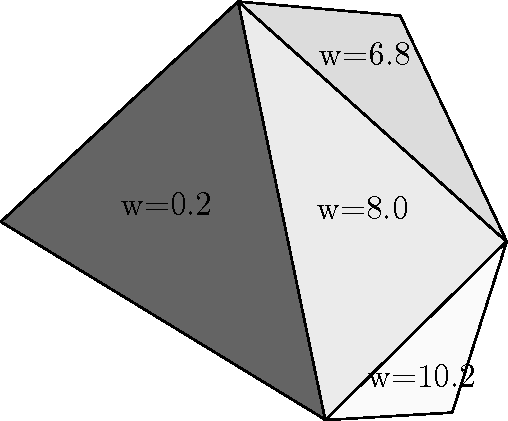
\includegraphics[width=0.21\columnwidth]{./img//mooving_orig}&
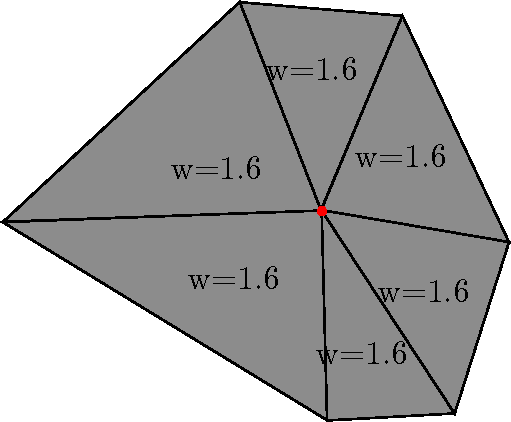
\includegraphics[width=0.21\columnwidth]{./img//mooving_avg}&
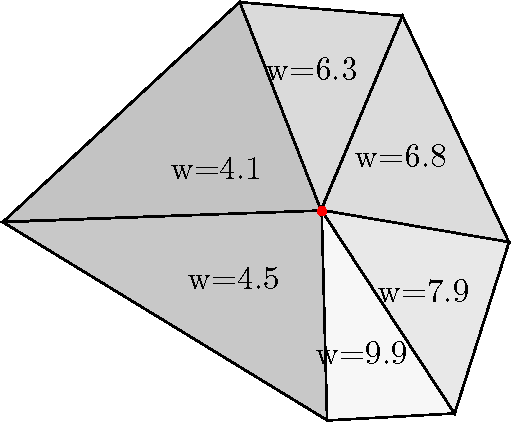
\includegraphics[width=0.21\columnwidth]{./img//mooving_weighted_avg}&
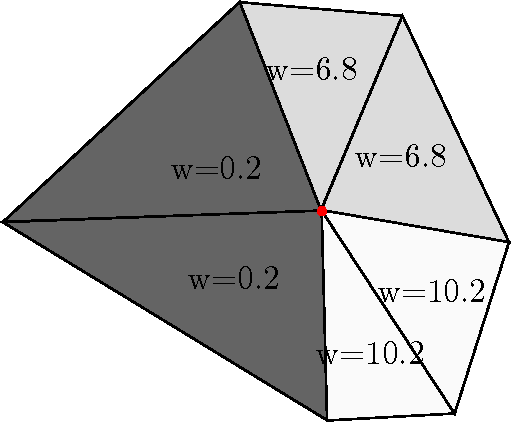
\includegraphics[width=0.21\columnwidth]{./img//mooving_min}\\
(a) & (b) & (c) & (d)\\
\end{tabular}
\end{center}
\caption{2D example of moving point addition in the new position after point removal (a brighter region corresponds to a higher weight, i.e., higher probability to be carved).}
\label{fig:reconstrEx_2}
\end{figure}

In case of very sparse data, the centroids of big tetrahedra, together with the associated visibility information, can be far from the newly added or moved points, and our update policy might lead to results far from the ideal solution, i.e., the straightforward approach discussed in Section \ref{subsec:straightforward_way}. Our algorithm overcomes this issue thanks to the use of the (so called) Steiner points added to the triangulation before the actual reconstruction is performed; this idea was already introduced in \cite{litvinov_lhuillier_13}.
We add Steiner points to the Delaunay triangulation every 5m along each axis so that they cover all the space that can be represented. The use of Steiner points limits the creation of very big tetrahedra, the visibility information becomes always local, and the update policy avoids drifts. Indeed, experimental results show good accuracy on varied scenes, even when lack of textures induces very sparse data.


\subsubsection{Complexity}
The complexity of the steps of our algorithm are reported in Table \ref{tab:ComStraight}. The main difference with respect to the straightforward algorithm is the replacement of the Rays removal to the weight update and backward casting which are the key of the gaining in computational complexity.
The proposed algorithm is thus $O(F\cdot N^2)$, so, in principle, the dependence with $F$ still remains and results in a non scalable solution. 

\subsubsection{Window Heuristic}
\label{subsub:window}
We are able to bound the complexity of our algorithm to $O(N^2)$ thanks to the following heuristic: instead of backward casting all the rays connecting the moving point to all the viewing cameras, we consider only the most recent cameras.
In this case the complexity of the ray casting becomes  $O(W\cdot N^2)$, where $W$ is the (constant) size  of the window (in our case $W = 15$), so the final complexity is $O(N^2)$.

%----------------------------------------------------------------------------------------------------------------------------
\section{Experimental validation}
\label{sec:experimental-results}
To evaluate our approach, we tested the system on four different sequences of the KITTI dataset \cite{Geiger_et_al12} on a 4 Core i7-2630QM CPU at 2.2Ghz (6M Cache), with 6GB of DDR3 SDRAM.
The video stream was captured by a Point Grey Flea 2, which records $1392\text{x}512$ gray scale images at $10$ fps. The vehicle pose are estimated through a RTK-GPS and they are the initial input of our system together with the video stream. 

Among all the sequences we choose the 0095 (268 frames) and 0104 (313 frames) since they depict two different urban scenarios: the former shows a narrow environment where the building fa\c{c}ades are close to the camera, the latter captures a wide road.
We also tested our approach on sequences 03 (801 frames) and 04 (271 frames) from the odometry dataset: these videos provide a varied landscape mixing natural (trees and bushes) and man-made (houses, cars) features.

 % $03:801frame(154kf) 04:271(48kf) 0095:268(48kf) 0104:313(56kf)

\begin{figure}[t]
\centering
\begin{tabular}{cc}
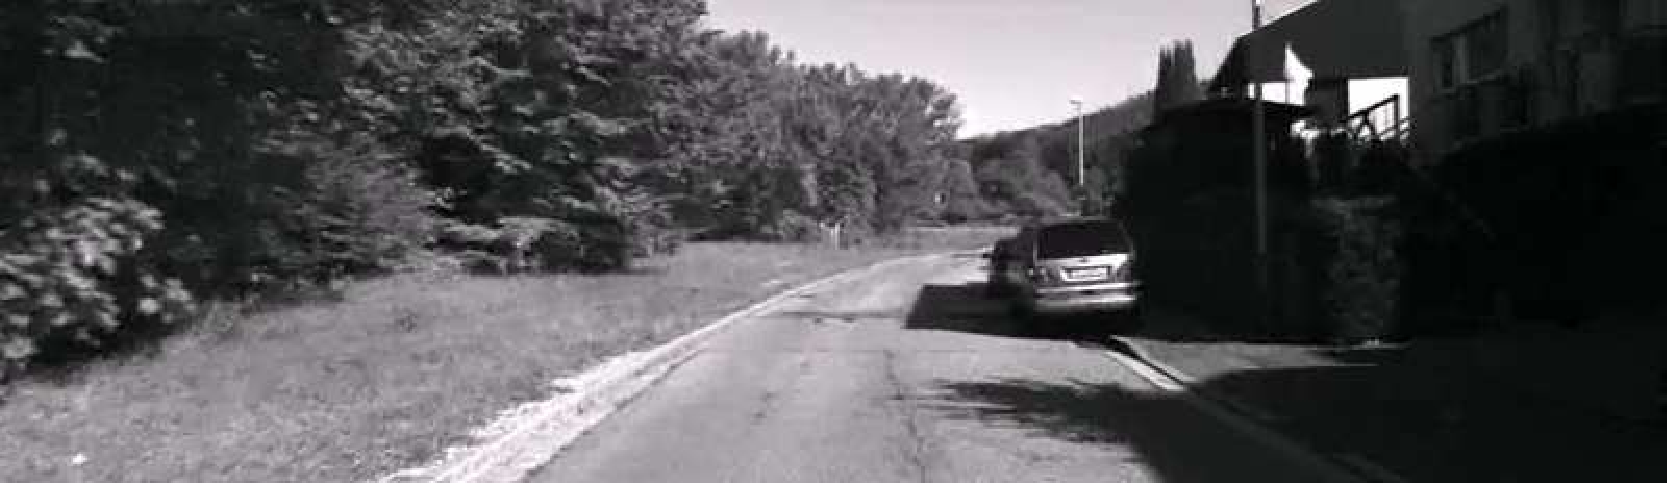
\includegraphics[width = 0.48\textwidth]{./img//ExRec_cropped}&
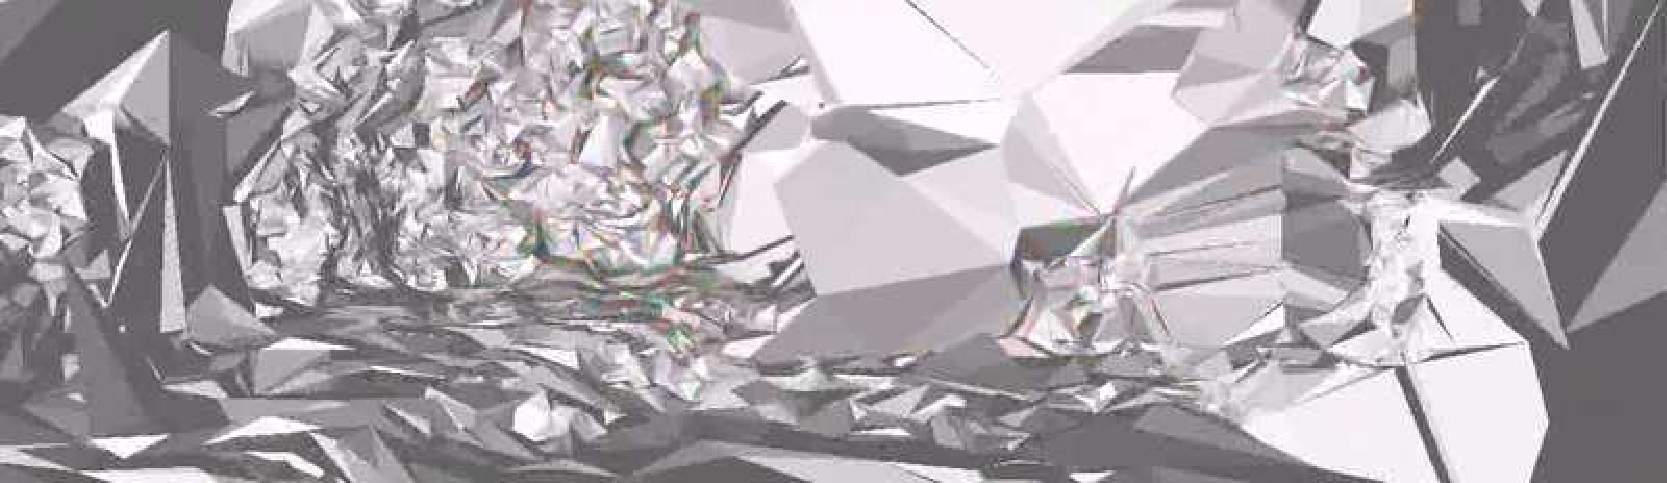
\includegraphics[width = 0.48\textwidth]{./img//ExRec01_cropped}\\
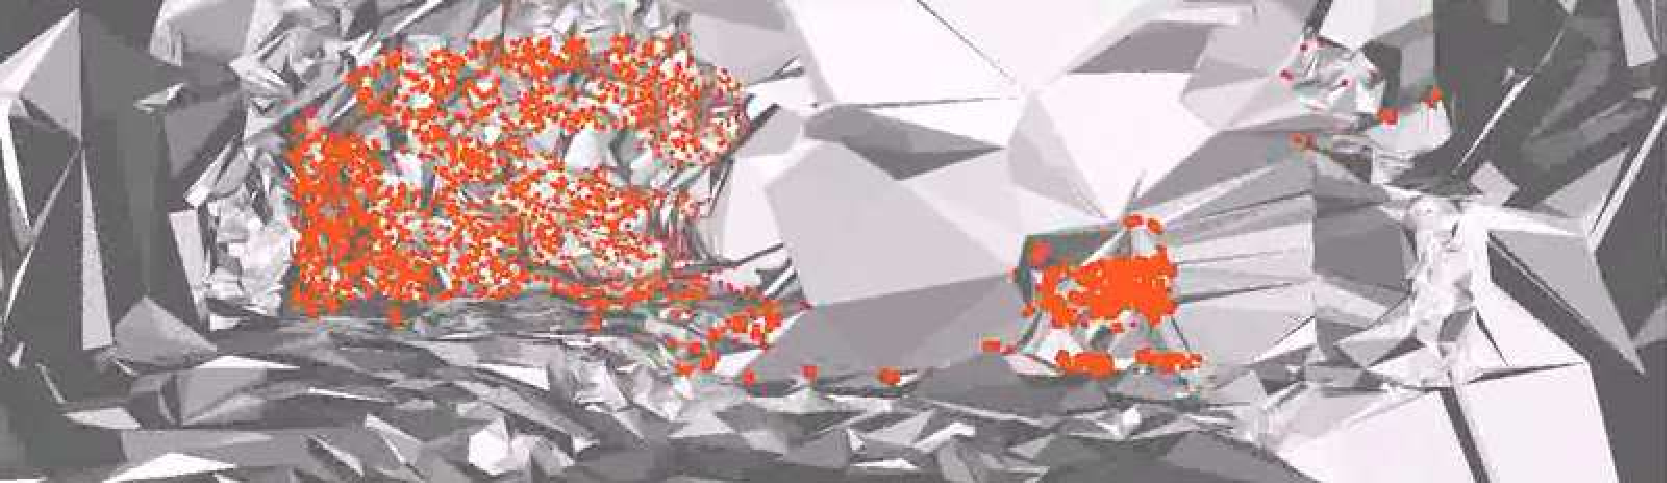
\includegraphics[width = 0.48\textwidth]{./img//ExRec02_cropped}&
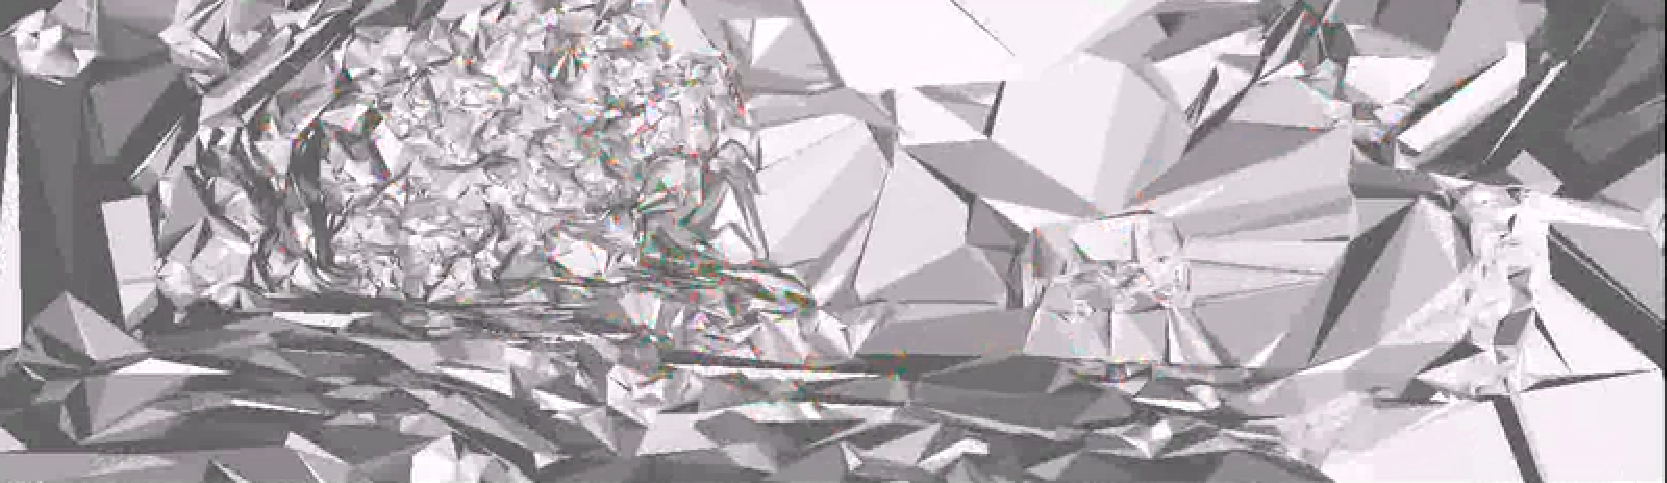
\includegraphics[width = 0.48\textwidth]{./img//ExRec05}\\
\end{tabular}
\caption{Incremental reconstruction example. From up left to bottom right: original frame, before point positions update, points moved in the scene (red dots) and  manifold updated.}
\label{fig:exampleFr}
\end{figure}

% \begin{figure}[t]
% \centering
% \begin{tabular}{cc}
% 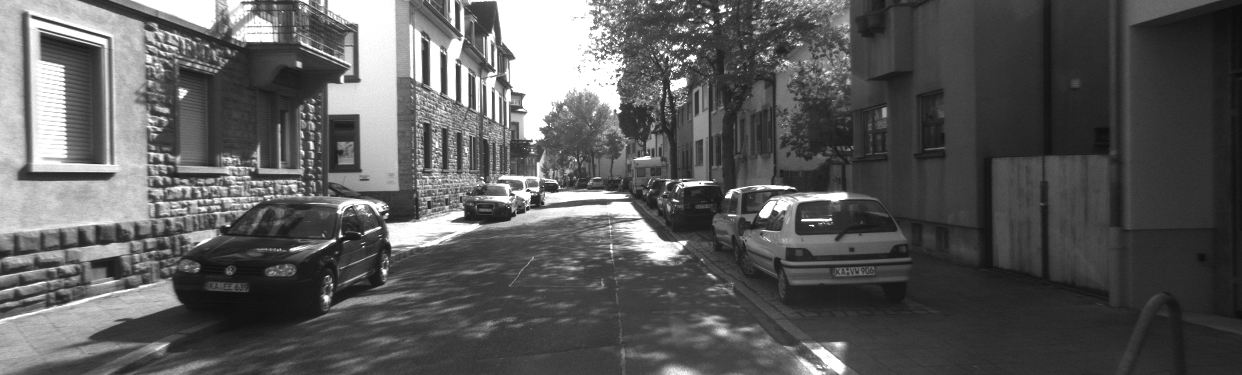
\includegraphics[width = 0.49\textwidth, height= 0.18\columnwidth]{./img//0095example}&
% 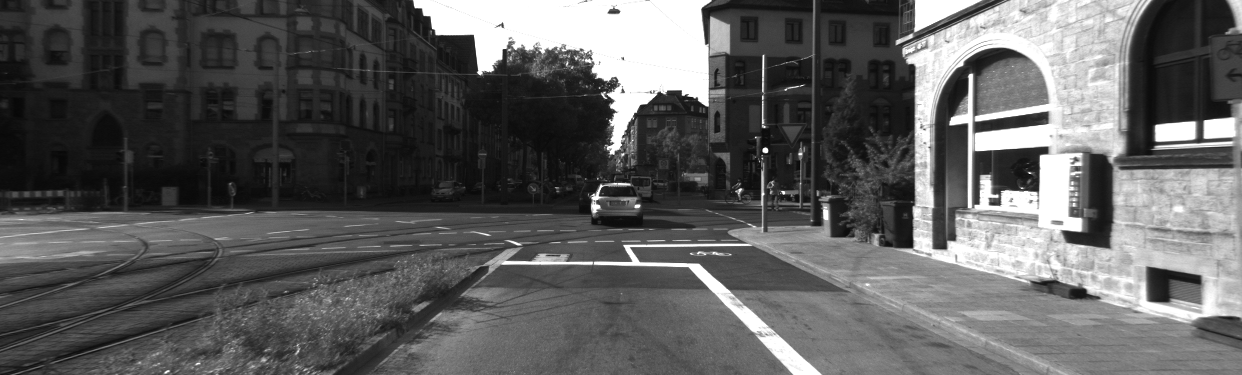
\includegraphics[width = 0.49\textwidth, height= 0.18\columnwidth]{./img//0104example}\\
% (a) Sequence 0095&
% (b) Sequence 0104\\
% 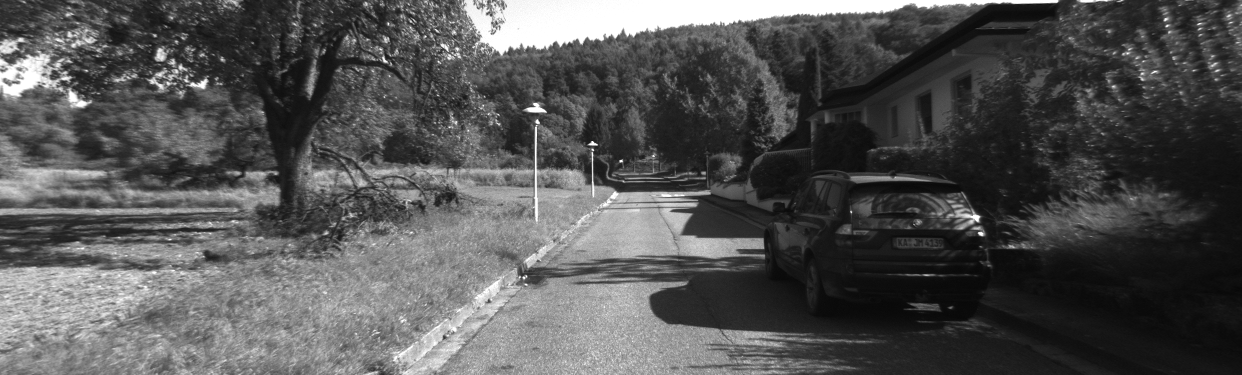
\includegraphics[width = 0.49\textwidth, height= 0.18\columnwidth]{./img//03example}&
% 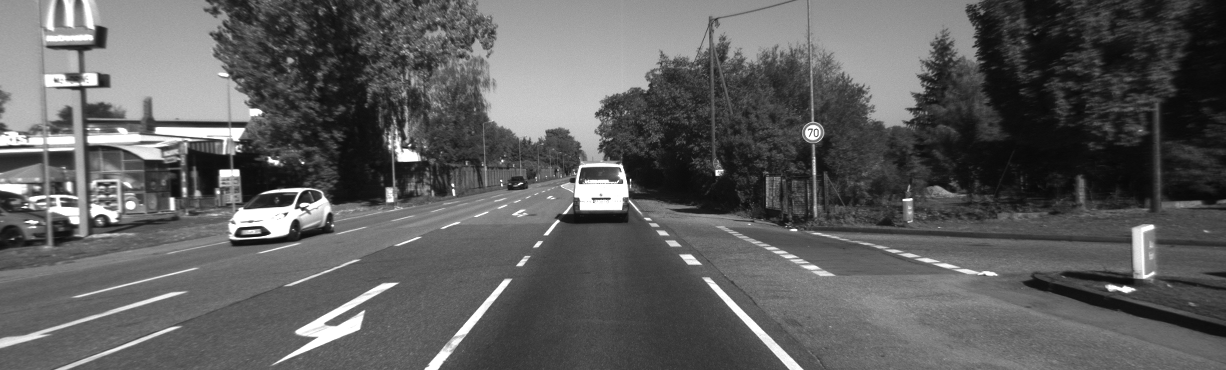
\includegraphics[width = 0.49\textwidth, height= 0.18\columnwidth]{./img//04example}\\
% (a) Sequence 03&
% (b) Sequence 04\\
% \end{tabular}
% \caption{Illustrative frames of the four sequences}
% \label{fig:exampleFr}
% \end{figure}

To provide a quantitative evaluation we compared the reconstructed meshes with the very accurate point clouds measured by the Velodyne HDL-64E sensor in the KITTI dataset through the CloudCompare tool \cite{CloudCompare}.
This tool computes the reconstruction error as the average of the distances between each Velodyne point and the nearest triangle in the reconstructed mesh.

We evaluated the performance and the accuracy of the Lovi's approach against our three different updating policy.
As explained previously, no manifold incremental reconstruction approach deals with moving points, so a fair comparison results to be between the straightforward approach of Lovi, applied to manifold reconstruction (Section \ref{subsec:straightforward_way}) and our updating policies. In Fig. \ref{fig:exampleFr} we show an example of the reconstruction results before and after the red points has been moved in the Delaunay triangulation (see also the video at \url{http://youtu.be/_-q9sKjcOC0}).

Fig. \ref{tab:results} shows the results of the comparison where we applied the window heuristic (Section \ref{subsub:window}) to all the algorithms. In the case of Lovi's algorithm we applied the forgetting heuristic with $K=5$ and $K=1$, where $K$ is the number of viewing rays stored for each tetrahedron.
Fig.  \ref{tab:results}(a) shows that the accuracy of the proposed approach, i.e, moving point management through minimum distance weight updates, is comparable with respect to Lovi's proposal outcomes, where the algorithm with $K=5$ stores more information, so it performs better.
We compared our approach with respect to Lovi's method instead of the other incremental reconstruction algorithm presented in \cite{litvinov_lhuillier_13}; the reasons are twofold. 
In \cite{litvinov_lhuillier_13} Litvinov and Lhuiller does not deal with moving points, which is the main point addressed in this paper. Moreover, Litvinov and Lhuiller point out in \cite{litvinov_Lhiuller14} that the ideal solution for a manifold reconstruction algorithm is represented by the manifold including as much as free space tetrahedra as possible. Since the solution provided by Lovi et al. coincides with the (non-manifold) mesh containing all the free space tetrahedra, a reconstruction accuracy similar to Lovi's suggests that the reconstruction is near to the ideal solution. In some cases our algorithm reaches even better accuracy, this is due to the smoothing effect induced by our heuristic.


Fig. \ref{tab:results}(a) shows that the Minimum Distance always outperforms the other two updating schema as expected (see the Section \ref{subsec:efficient_way}).

In Fig. \ref{tab:results}(b) we report the time performance of the algorithms.
Let $T_{\text{mov}}$ and $T_{\text{non-mov}}$ be the overall processing time with and without moving points, and $N_{\text{mov}}$ be the number of the total points moves, e.g., if one point moves three times, $N_{\text{mov}}=3$.
The overhead introduced in the whole reconstruction process for each move of each point has been computed as $\frac{T_{\text{mov}} - T_{\text{non-mov}}}{N_{\text{mov}}}$.
The performance of the different update schema we presented in Section \ref{subsec:efficient_way} is very similar since the steps involved are basically the same: for each update on the Delaunay data structure, we iterate over the old tetrahedra to collect the weights, then we iterate over the new tetrahedra to set the new weights.
As expected by Section \ref{subsec:efficient_way}, our algorithm clearly outperforms Lovi's approach. Our updating schema is very efficient for two reasons. 
First, we only need to update locally the visibility, while Lovi's approach casts a ray for each visibility ray stored inside the tetrahedra.
Second, when we remove a point (first step of moving point management), we perform a ray casting backward to update only the convenient tetrahedra,  instead of iterating over the whole triangulation to remove the visibility rays involving the point moved as in \cite{Lovi_et_al_11}.
  
 
\begin{figure}[t]
\centering
  \begin{tabular}{ccc}
    \centering
    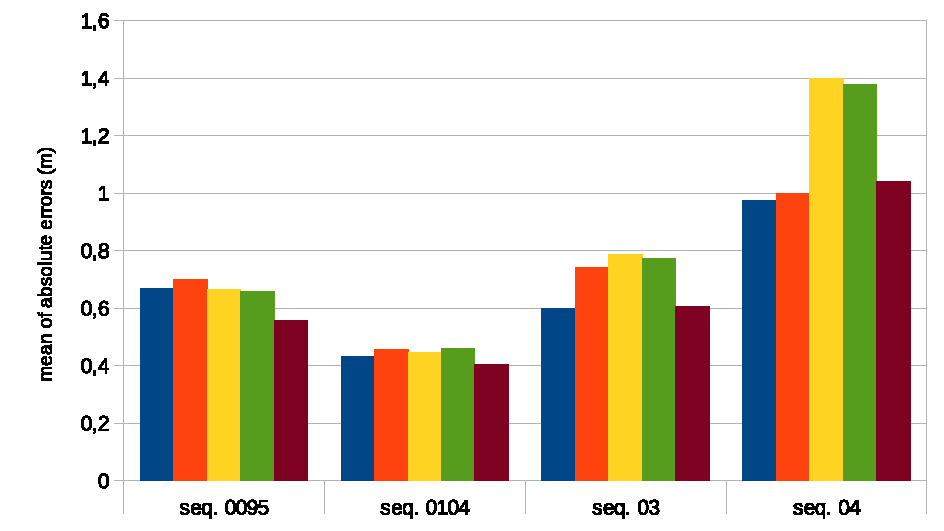
\includegraphics[height=0.25\textwidth]{././img//results.pdf}&
    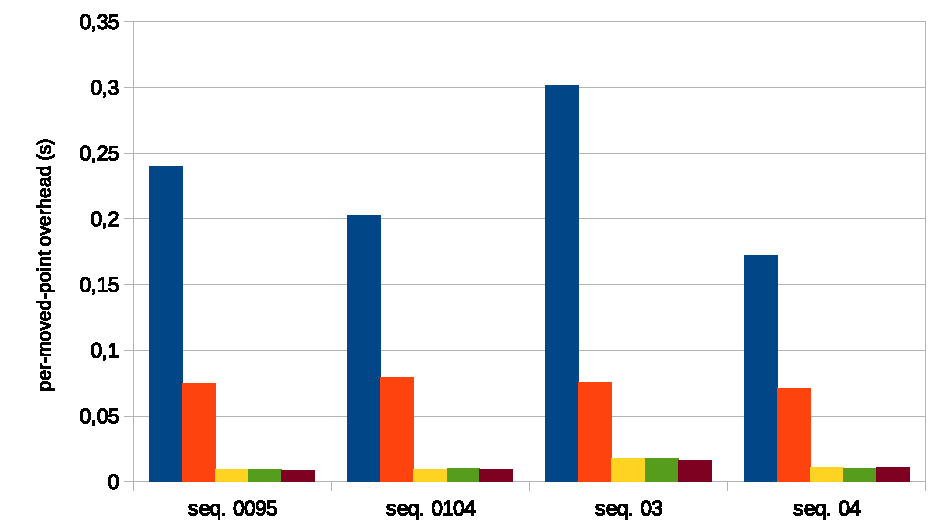
\includegraphics[height=0.25\textwidth]{././img//resultsTiming.pdf}&
    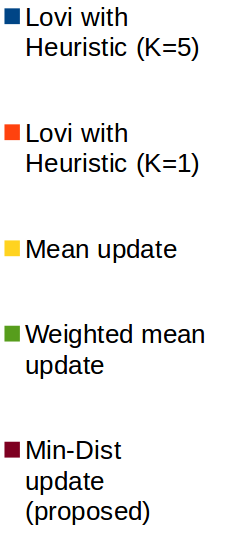
\includegraphics[height=0.22\textwidth]{././img//legenda}\\
    (a) Absolute errors (m).&
    (b) Per-point overhead (s).&\\
  \end{tabular}
  \caption{Experimental evaluation of the proposed approach with respect to Lovi's \cite{Lovi_et_al_11}.}
   \label{tab:results}
\end{figure}


%----------------------------------------------------------------------------------------------------------------------------
\section{Conclusion and future work}
\label{sec:conclusion}
In this paper we have shown that manifold reconstruction from sparse data with moving points is not a trivial task. To keep the Delaunay property valid when a point moves inside the Delaunay triangulation, we have to remove it and add a new point in the new position. This induces the removal of a set of tetrahedra, with the associated visibility information; then, we have to add a new set of tetrahedra with coherent visibility information; finally we have to update the visibility information in all the tetrahedra affected by the point move.

Existing solutions successfully applied for classic Space Carving, result to be inefficient and slow when applied in the manifold reconstruction setting. 
In this setting, we investigated different approaches to handle visibility information propagation, by updating the weight for each tetrahedron, which roughly represents  the number of ray intersections, and we proposed an efficient algorithm to conveniently update it. 
We tested our system with the KITTI dataset and it clearly outperforms the existing approach of Lovi et al. \cite{Lovi_et_al_11} for incremental manifold reconstruction.

Future works would include a photometric refinement of the manifold extracted incrementally, and an evaluation of the manifold quality on-the-fly, relying on the uncertainty information carried by the estimation of 3D points. 
A natural extension could also deal with the reconstruction of non-rigid shapes whose 3D points are moving.


% 
% 
% \section{Experimental results}
% \label{sec:experimental-results}
% A monocular 3D reconstruction benchmark for urban scenarios, with accurate ground truth, does not exist; then we evaluated our contribution on four different sequences of the public available dataset \cite{Geiger_et_al12}. 
% This dataset contains a Velodyne HDL-64E point cloud for each sequence which can be used as ground truth for 3D reconstruction validation.
% The video stream was captured by a Point Grey Flea 2 camera, which took $1392\text{x}512$ gray scale images at $10$ fps and its view point was directed towards the direction of the vehicle motion. 
% The vehicle and camera poses are estimated by a RTK-GPS and they are the initial input of our system together with the video stream.
% 
% Among all the KITTI sequences we choose the 0095 (268 frames) and 0104 (313 frames) from the raw dataset and, sequences 03 (801 frames) and 04 (271 frames) from the odometry dataset. 
% They depict four different urban scenarios: the 0095 shows a narrow environment where the building fa\c{c}ades are close to the camera, the 0104 captures a wide road, while the 03 and 04 sequences provide a varied landscape mixing natural (trees and bushes) and man-made (houses, cars) features.
% We run the tests on a 4 Core i7-2630QM CPU at 2.2Ghz (6M Cache) with 6GB of DDR3 SDRAM. To have a qualitative overview of the results we refer the reader to the video in the supplementary material. 
% 
% 
% \begin{figure}[t]
%   \centering
%   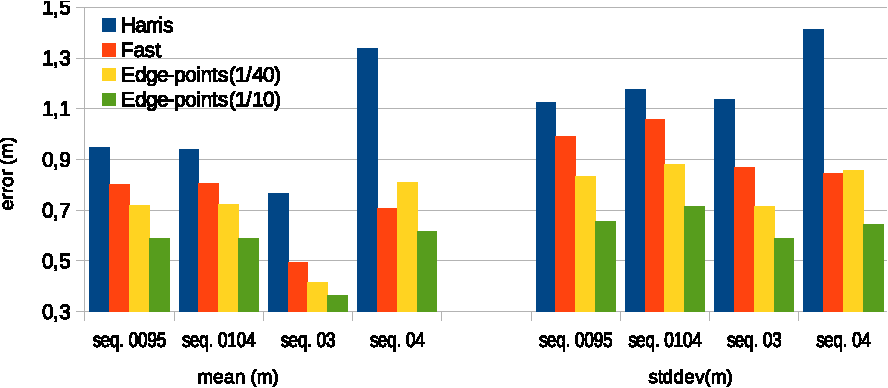
\includegraphics[width=0.43\textwidth]{././img//risultati.pdf}
%   \caption{Reconstruction absolute errors of the proposed algorithm (Edge-Point) versus two classical feature based 3D reconstruction (Harris, FAST).}
%    \label{tab:comp}
% \end{figure}
% 
% To provide a quantitative evaluation we compared the reconstructed meshes with the very accurate point clouds measured by the Velodyne of the KITTI dataset through the CloudCompare tool \cite{CloudCompare}.
% This tool was used to compute the reconstruction error, i.e., the average of the distances between each Velodyne point and the nearest mesh triangle.
% Fig. \ref{tab:comp} shows the comparison, on the same dataset, between the reconstruction with the proposed Edge-Points cloud and the reconstruction with the FAST and the Harris corner point clouds as in \cite{litvinov_Lhiuller14}.  
% We adopted two different edge downsampling rate (low $\frac{1}{40}$ and high $\frac{1}{10}$) to verify that the accuracy gain was not a matter of number of reconstructed features, but it was due to the better choice. 
% Indeed, Table \ref{tab:reconstrPt} shows that, even if the reconstructed Edge-Points with low downsampling rate are significantly less than the reconstructed points using classical features, the accuracy of the manifold estimated in the former case is always better with except to one case (sequence 04 with respect to FAST).  
% The good fitting of the Edge-Points to the real 3D curves, lets the reconstructed surface to lay closer to the real one; this allows our Edge-Point reconstruction approach to outperform reconstructions upon non-Edge-Points.
% Fig. \ref{fig:distr} shows how Edge-Points have a more homogeneous distribution on the images, with respect to the other features: we subdivided the images of the sequence into a 3x5 grid and we report the percentage of extracted features for each cell.
% 
% 
% \begin{figure}[t]
%   \centering
%   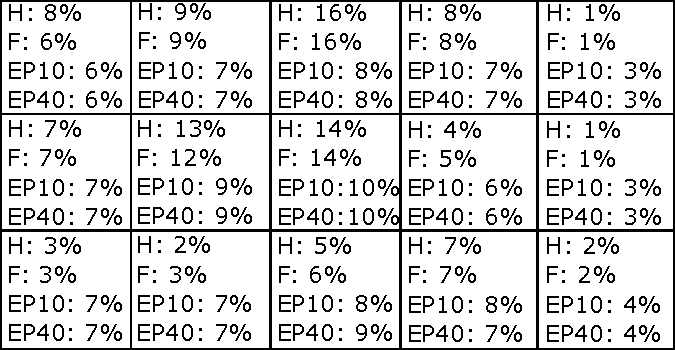
\includegraphics[width=0.4\textwidth,height=0.18\textwidth]{././img//distribution}
%   \caption{Distribution of Harris corner (H), FAST (F) and Edge-Points with downsampling $\frac{1}{10}$ (EP10) and $\frac{1}{40}$ (EP40) on the 0095 sequence.}
%    \label{fig:distr}
% \end{figure}
% 
% 
% To understand how Edge-Points extraction, tracking, filtering and estimation affect the performance of our reconstruction algorithm we reported the timing in Fig. \ref{tab:timing} for Edge-Points with downsampling rate $\frac{1}{10}$.
% In our experiments, the tracking, filtering and estimation processing times were proportional to the number of extracted features, while the extraction depends on the selected features: the mean per-frame times are 0.0044s (Harris),  0.0010s (FAST),  0.0036 (Edge-Points with $\frac{1}{40}$ downsampling),  0.0037 (Edge-Points with $\frac{1}{10}$ downsampling). FAST is the fastest feature to extract but the impact of this step on the overall 3D estimation pipeline is almost negligible (1\% to 3\% of the pipeline).
% 
% 
% 
% \begin{table}[t]
%   \caption{Mean number of reconstructed (and extracted) points per keyframe.}
%   \scriptsize
%    \label{tab:reconstrPt}
%    \centering
%    \begin{tabular}{p{0.2\columnwidth}cccc}
%    \toprule 
%                                               & 0095            & 0104        &  03         & 04   \\
%    \hline   
%    {Harris}                                   & 423 (2556)      & 561 (2979)  & 946 (3342)  & 692 (2036) \\
%    %\hline
%    {FAST}                                     & 550 (3463)      & 865 (3950)  & 1215 (4358) & 953 (2850) \\
%    %\hline
%   {Edge-Point (${1}/{40}$ downs.)}   & 165 (1327)      & 267 (1485)  & 404 (1650)  & 382 (1277) \\
%    %\hline
%    {Edge-Point (${1}/{10}$ downs.)}  & 656 (5310)      & 946 (5938)  & 1615 (6598) & 1524 (5106)  \\
%     \bottomrule
%   \end{tabular}
%   \end{table} 
%   
% % \begin{table}[t]
% %   \caption{Mean number of reconstructed (and extracted) points per keyframe.}
% %   \footnotesize
% %    \label{tab:reconstrPt}
% %    \centering
% %    \begin{tabular}{p{0.25\columnwidth}cccc}
% %    \toprule 
% %                                               & 0095    & 0104    & 03      & 04   \\
% %    \hline   
% %    {Harris}                                   & 301     & 300 ()     & 112     & 151 \\
% %    %\hline
% %    {FAST}                                     & 1291    & 1322 (3950)    & 1732    & 1152 \\
% %    %\hline
% %   {Edge-Point (${1}/{40}$ downsample rate)}   & 447     & 521  (2979)   & 266     & 467 \\
% %    %\hline
% %    {Edge-Point (${1}/{10}$ downsample rate)}  & 1785    & 2077 (5938)   & 1062    &1858  \\
% %     \bottomrule
% %   \end{tabular}
% %   \end{table} 
% In Table \ref{tab:numArtifacts} we show the effect of the Inverse Cone Heuristic. We manually counted the visually critical artifacts in the mesh reconstructed with and without the heuristic; in parenthesis, we reported the number of artifacts affecting the camera traversability path. The heuristic diminished significantly the number of artifacts by $68$\% up to $85$\%, depending on the sequence considered. 
% A fair comparison with the method in \cite{litvinov_Lhiuller14} is not possible, since their dataset and their code is not publicly available. We only point out that, in their experiments, they reported \cite{litvinov_Lhiuller14} an artifact removal rate of $35$\%.
% 
% 
% We are also able to provide a qualitative comparison about how the Inverse Cone Heuristic affects the performance of the reconstruction. The method in \cite{litvinov_Lhiuller14} takes $0.43$s per frame on a Xeon W3530 at 2.8Ghz (8M Cache), whose performances are very similar to our machine.  Our datasets are different, but depict a similar urban scenario, and our approach (Table \ref{tab:inverseTiming}) runs one to two order of magnitude faster, thanks to the CGAL \cite{cgal} triangulation data structure which enable very efficient access to  tetrahedra neighboring the ones traversed by the camera-to-point viewing rays. 
% Fig. \ref{fig:exampleArt} shows a mesh without and with the inverse cone heuristic; the big artifact occluding the camera trajectory in (a) disappears in (b).
%  
% 
% 
% \begin{figure}
% \centering
% \begin{tabular}{c}
% 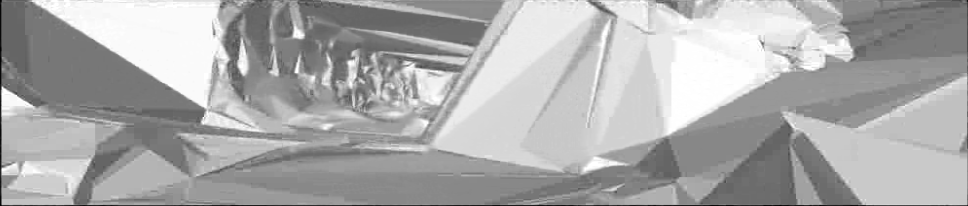
\includegraphics[width=0.7\columnwidth]{./img//inverseConeWithout}\\
% (a)\\
% 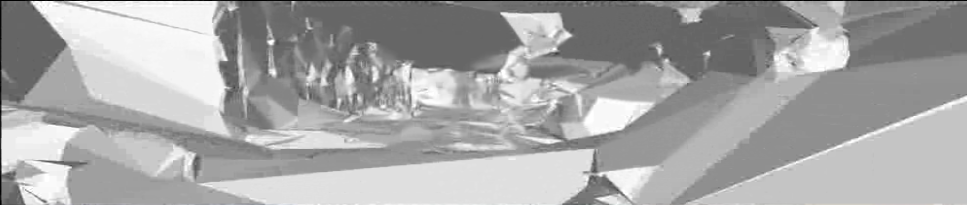
\includegraphics[width=0.7\columnwidth]{./img//inverseConeWith}\\
% (b) 
% \end{tabular}
% \caption{Example of preemptive artifact removal: (a) without  and (b) with the Inverse Cone Heuristic.}
% \label{fig:exampleArt}
% \end{figure}
% 
% % Finally, we are able to conclude that the Inverse Cone Heuristic is surely effective, moreover it is possible to apply it complementary to the algorithm presented in \cite{litvinov_Lhiuller14}, since it has a really low impact on the performances. 
% 
%  \begin{figure}[t]
%   \centering
%   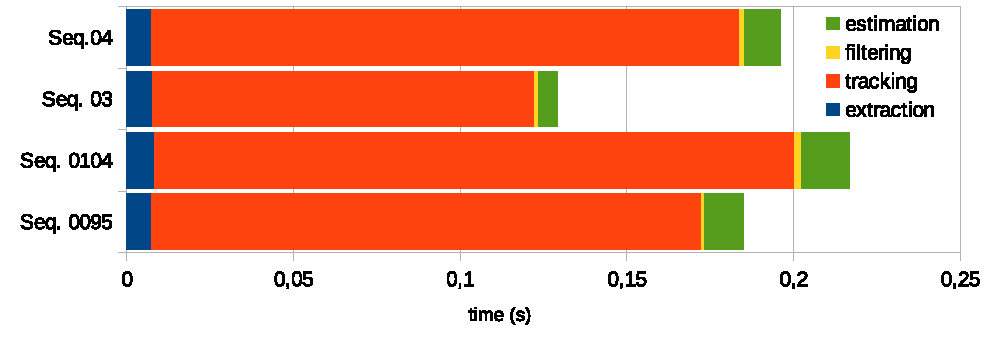
\includegraphics[width=0.4\textwidth]{././img//risultatitiming.pdf}
%   \caption{Per-frame time (in seconds) of Edge-Point estimation ($\frac{1}{10}$ downsampling rate).}
%    \label{tab:timing}
% \end{figure}
% %
% 
%   
% 
% %----------------------------------------------------------------------------------------------------------------------------
% \section{Conclusion and future works}
% \label{sec:conclusion}
% In this paper we have shown that Edge-Points represent a very convenient choice to build a 3D Delaunay triangulation for the Space Carving reconstruction, especially in urban scenarios.
% We have shown how to successfully reconstruct their 3D positions by tracking their successive projections in the video images and by filtering the results of the KLT tracker with simple constraints. On these reconstructed points we incrementally built a 3D triangulation to reconstruct a manifold surface with a novel version of the algorithm in \cite{litvinov_lhuillier_13} and \cite{litvinov_Lhiuller14} improved by means of the Inverse Cone Heuristic.
% 
% The results reached by our algorithm showed that in urban scenarios the Edge-Points estimation enables a detailed reconstruction, which is better then those obtained by  using only stable features, such as Harris or FAST corners.
% 
% 
% To deal with visual artifacts affecting the reconstructed manifold, we proposed a very fast method to preemptively avoid their creation. In the experiments the manifolds reconstructed with this heuristic are almost clear from visual artifacts.
% Future works involve the preemptive filtering of some of the Edge-Points not belonging to the real-world edges or laying in a very low parallax regions, and  the management of moving 3D points inside the Delaunay triangulation as in \cite{Romanoni15a}.
% 
% \begin{table}[t]
%   \caption{Number of artifacts w/o and w/ the Inverse Cone Heuristic. In parenthesis number of artifacts affecting the camera traversability path.}
%   \footnotesize
%    \label{tab:numArtifacts}
%    \centering
%    \begin{tabular}{p{0.25\columnwidth}cccc}
%    \toprule 
%                                & 0095  & 0104& 03 & 04   \\
%    \hline
% %    {w/o ICH }                 & 21&21& 40& 22\\
% %    w/  ICH                    & 4&3& 12& 7\\
% %    \% removed                 & 80&85& 70& 68\\
%    w/o ICH                 & 21 (4) &21(2)& 40(15)& 22(7)\\
%    w/  ICH                    & 4(0) &3(1)& 12(3)& 7(1)\\
%  \% removed                 & 80(100) &85(50)& 70(80)& 68(85)\\
%     \bottomrule
%   \end{tabular}
%   \end{table}
%   
% 
% 
% 
% \begin{table}[t]
%   \caption{Per-frame time (in seconds) of the Inverse Cone Heuristic (ICH) for preemptive artifacts removal.}
%   \footnotesize
%    \label{tab:inverseTiming}
%    \centering
%    \begin{tabular}{cccc}
%    \toprule  
%      0095  & 0104&03 & 04     \\
%    \hline
%      0.002 & 0.003& 0.010 & 0.001  \\
%     \bottomrule
%   \end{tabular}
%   \end{table} 